\chapter{Detekcia objektov v obraze}

    Pre niektoré techniky klasifikácie objektov je nutné najprv v obraze tieto objekty nájsť. Existuje k tomu veľké množstvo metodík, pri čom každá z nich má svoje výhody a nevýhody. Je teda nutnosťou zistiť, ktorá metóda najviac vyhovuje použitiu pre túto prácu. Je nutnosťou zvoliť jednoduchšie medódy vzhľadom na výpočtový výkon zariadenia.

\section{Prahovanie}

    Prahovanie je jasová transformácia, pri ktorej je šedotónový obraz rozdelený na dve a viac oblastí podľa jasovej úrovne pixelov. O tom, do ktorej z oblastí je daný pixel priradený rozhoduje prah, ktorého hodnotu je treba určiť. Výsledkom je obraz s len dvomi úrovňami jasu - binárny obraz.

    Pri~správnom predspracovaní obrazu prahovaním je možné v~ňom jednoducho oddeliť objekty od~pozadia v~prípade,ak sa jas objektu dostatočne líši od jasu pozadia. Ak sa však jasové hodnoty objektu a pozadia príliš podobajú, nemusí existovať dostatočne robustné určenie prahu oddeľujúceho objekty od pozadia. \cite{Morse1998/1} \cite{Buhl2023}

    Prevod farebného obrazu do šedotónového s cieľom získať pre každý pixel jednu hodnotu jasu je možný nie len výpočtom priemerného jasu farebných zložiek pixelu, ale aj ich lineárnou kombináciou s váhami určenými podľa predpokladanej farby pozadia. V prípade detekcie objektov na oblohe, ktorá tvorí pozadie prevažne modrej farby, dáva zmysel uvažovať modrú farbu s vyšším významom. Vďaka tomu môžu byť zvýraznené objekty, ktorých farba sa lýši od modrej farby pozadia. Inou možnosťou je uvažovať len jednu farebnú zložku, teda modrú, čím by bol ušetrený výpočtový výkon pred tým využitý pri výpočte súčtov zložiek.

    \begin{figure}[!ht]
        \begin{center}
            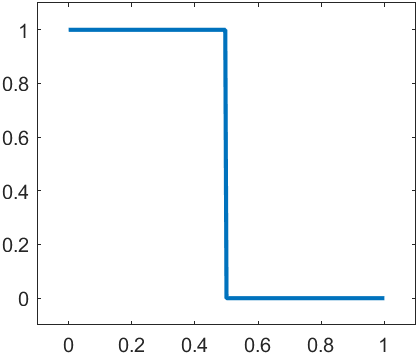
\includegraphics[scale=.4]{obrazky/threshold/thresholding.png}
        \end{center}
        \caption{Funkcia prahovania s prahom 0.5 pre svetlé pozadie}
    \end{figure}

\subsection{Globálne prahovanie}

    Globálne prahovanie je často používaná technika, pri ktorej je použítý jediný prah na celý obraz, čo nemusí byť vhodné v~prípade, ak je jasová úroveň pozadia rôzna v~rôznych miestach obrazu. \cite{Morse1998/1}

    \begin{itemize}
        \item \textbf{Jednoduché prahovanie} je technika, pri ktorej je globálny prah určený dopredu ručne. V prípade, že sa jasová úroveň pozadia v čase mení, je vhodnejšie použiť techniky s adaptívnym nastavením prahu.

        \item Prahovanie \textbf{podľa známeho rozloženia} predpokladá že poznáme relatívnu veľkosť oblasti, ktorú zaberá pozadie v obraze. Ak vieme, že objekt je svetlejší ako pozadie, môžeme určiť prah z kumulatívneho histogramu tak, aby relatívny počet pixelov pod úrovňou prahu bol rovnaký ako oblasť, ktorú má zaberať pozadie.

        \item Algoritmus \textbf{K-Means} (K priemerov) pre zhlukovú analýzu rozdeľuje dáta do skupín s cieľom minimalizovať vzdialenosť bodov v zhluku a maximalizovať vzdialenosť medzi zhlukmi. Jedná sa o algoritmus učenia bez učiteľa. Funguje na princípe iterovaného posúvania \emph{k} stredov zhlukov (v prípade binárneho prahovania je \emph{k = 2}) smerom k priemeru hodnôt priradenému danému stredu v aktuálnom kroku.

        \item \textbf{Otsuova metóda} automatického určenia prahu je založená na maximalizovaní vzájomnej odchýlky medzi triedami. Využíva normalizovaný kumulatívny histogram, z ktorého určuje vzájomný rozptyl pre všetky možné hodnoty prahu a vyberá ten optimálny.
    \end{itemize}

    \begin{figure}[!ht]
        \centering
        \begin{tikzpicture}[>=stealth, node distance=5cm]
            \node (image1) {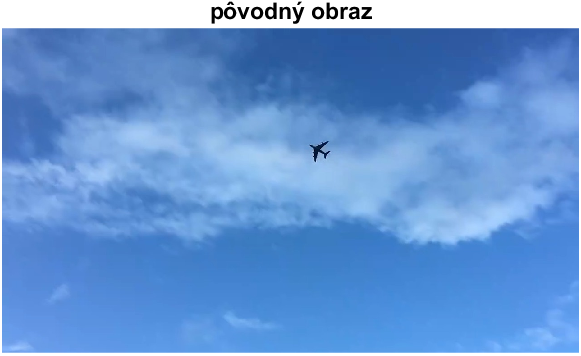
\includegraphics[width=.3\textwidth]{obrazky/threshold/img.png}};
            \node (image2) [right of=image1] {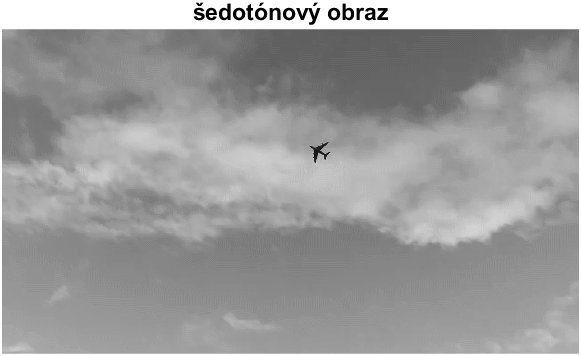
\includegraphics[width=.3\textwidth]{obrazky/threshold/img_gray.png}};
            \node (image3) [right of=image2] {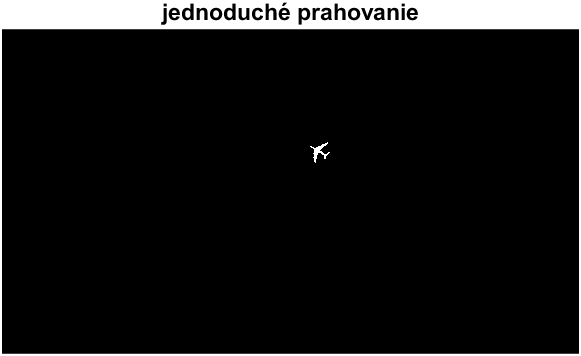
\includegraphics[width=.3\textwidth]{obrazky/threshold/img_simple_thresh.png}};

            \draw[->] (image1) -- (image2) node[midway, above] {};
            \draw[->] (image2) -- (image3) node[midway, above] {};
        \end{tikzpicture}
        \begin{tikzpicture}[>=stealth, node distance=5cm]
            \node (image1) {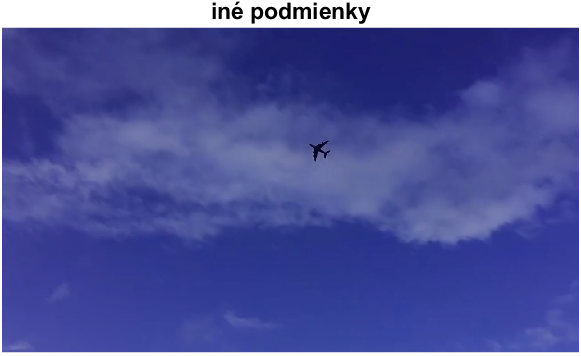
\includegraphics[width=.3\textwidth]{obrazky/threshold/img_dark.png}};
            \node (image2) [right of=image1] {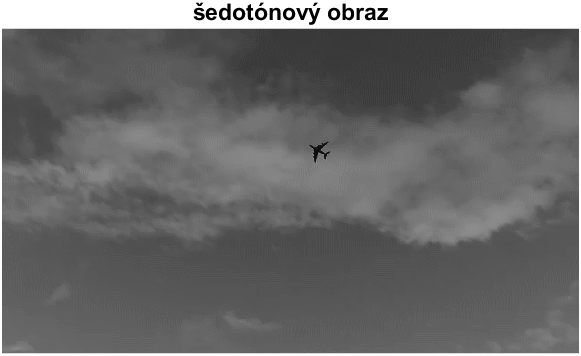
\includegraphics[width=.3\textwidth]{obrazky/threshold/img_dark_gray.png}};
            \node (image3) [right of=image2] {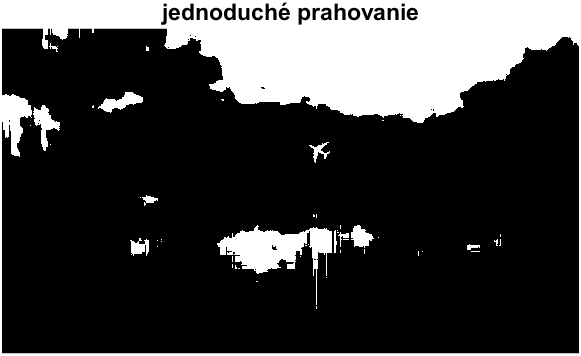
\includegraphics[width=.3\textwidth]{obrazky/threshold/img_dark_simple_thresh.png}};

            \draw[->] (image1) -- (image2) node[midway, above] {};
            \draw[->] (image2) -- (image3) node[midway, above] {};
        \end{tikzpicture}
        \caption{Jednoduché prahovanie}
    \end{figure}

    \begin{figure}[!ht]
        \centering
        \begin{tikzpicture}[>=stealth, node distance=5cm]
            \node (image1) {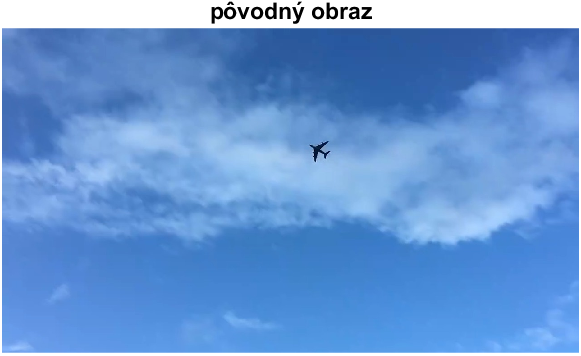
\includegraphics[width=.3\textwidth]{obrazky/threshold/img.png}};
            \node (image2) [right of=image1] {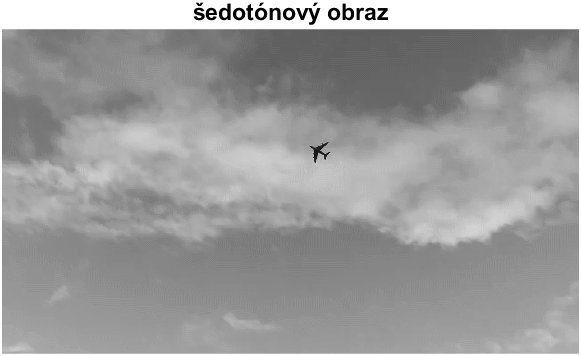
\includegraphics[width=.3\textwidth]{obrazky/threshold/img_gray.png}};
            \node (image3) [right of=image2] {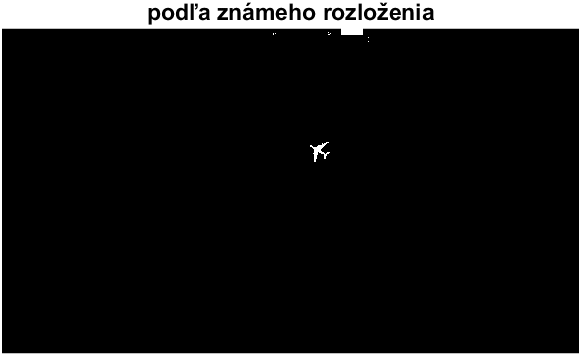
\includegraphics[width=.3\textwidth]{obrazky/threshold/img_thresh_distr.png}};

            \draw[->] (image1) -- (image2) node[midway, above] {};
            \draw[->] (image2) -- (image3) node[midway, above] {};
        \end{tikzpicture}
        \begin{tikzpicture}[>=stealth, node distance=5cm]
            \node (image1) {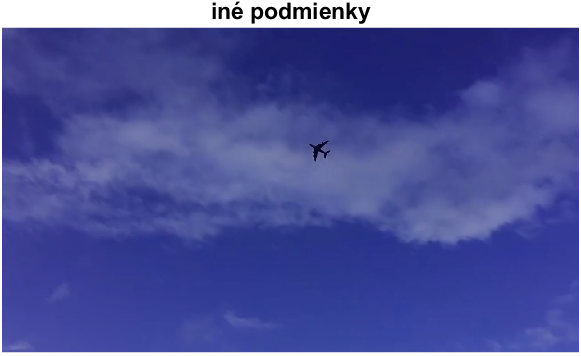
\includegraphics[width=.3\textwidth]{obrazky/threshold/img_dark.png}};
            \node (image2) [right of=image1] {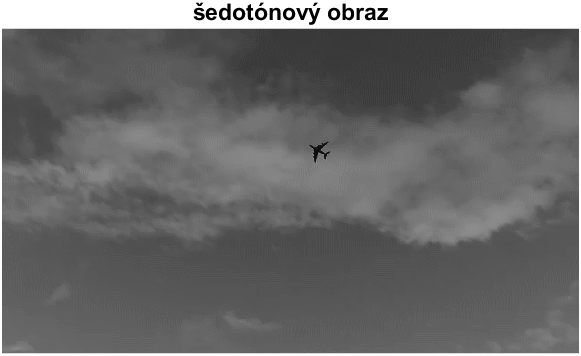
\includegraphics[width=.3\textwidth]{obrazky/threshold/img_dark_gray.png}};
            \node (image3) [right of=image2] {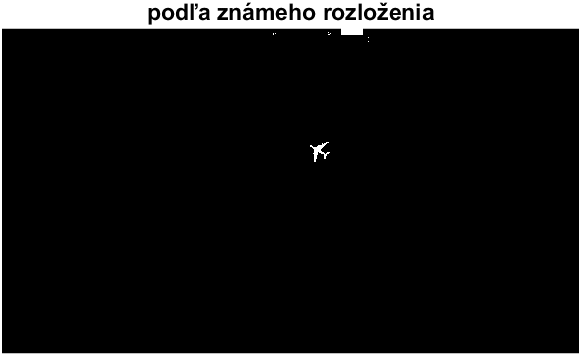
\includegraphics[width=.3\textwidth]{obrazky/threshold/img_thresh_distr.png}};

            \draw[->] (image1) -- (image2) node[midway, above] {};
            \draw[->] (image2) -- (image3) node[midway, above] {};
        \end{tikzpicture}
        \caption{Automatické prahovanie (podľa známeho rozloženia)}
    \end{figure}

\subsection{Lokálne prahovanie}

    V prípade, že je jas pozadia rôzny v rôznych častiač obrazu, je vhodné určiť hodnotu prahu z jasovej úrovne okolia každého prahovaného pixelu. Toto takzvané adaptívne prahovanie má síce vyššiu výpočtovú náročnosť ako jednoduchšie globálne prahovanie, keďže je nutné určiť prah pre každý bod obrazu samostatne, je však robustnejšie voči nevhodnému pozadiu. \cite{Buhl2023}

    \begin{figure}[!ht]
        \centering
        \begin{tikzpicture}[>=stealth, node distance=5cm]
            \node (image1) {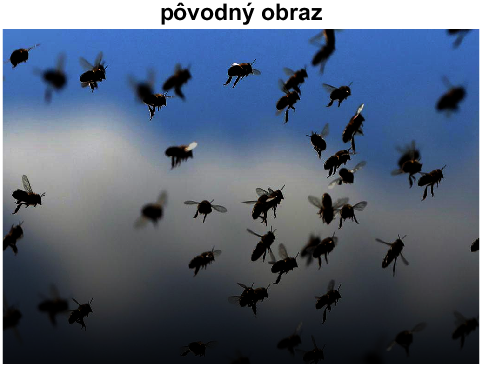
\includegraphics[width=.3\textwidth]{obrazky/threshold/img2.png}};
            \node (image2) [below of=image1] {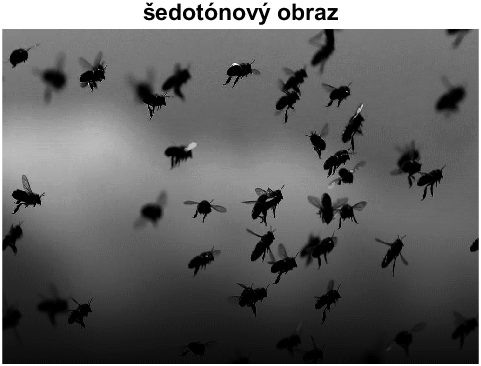
\includegraphics[width=.3\textwidth]{obrazky/threshold/img2_gray.png}};
            \node (image3) [left of=image2] {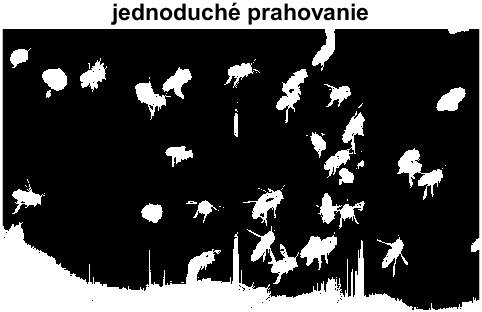
\includegraphics[width=.3\textwidth]{obrazky/threshold/img2_simple_thresh.png}};
            \node (image4) [right of=image2] {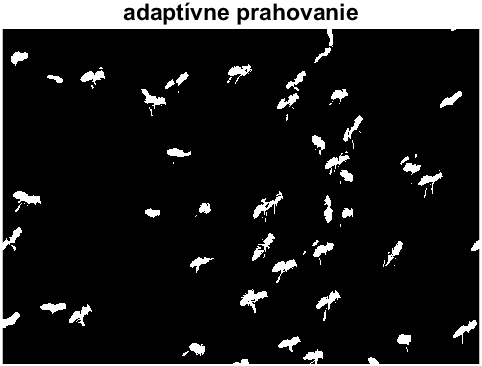
\includegraphics[width=.3\textwidth]{obrazky/threshold/img2_adaptive_thresh.png}};

            \draw[->] (image1) -- (image2) node[midway, above] {};
            \draw[->] (image2) -- (image3) node[midway, above] {};
            \draw[->] (image2) -- (image4) node[midway, above] {};
        \end{tikzpicture}
        \caption{Adaptívne prahovanie (podľa známeho rozloženia)}
    \end{figure}

\section{Detekcia hrán}

    Ako jednu z metód vyhľadávania objektov v obraze je možné využiť obraz hrán a~vyhľadať v ňom kontúry objektov. Opäť existuje niekoľko spôsobov, ako získať obraz hrán a ako ho využiť k segmentácii obrazu, teda k detekcii objektov.

    Na vytvorenie obrazu hrán z nasnímaného obrazu sa používa konvolúcia obrazu s operátorom navrhnutým tak, aby aproximovalo deriváciu určitého rádu. Medzi často používané operátory patria Prewittov a Sobelov operátor, ktoré aproximujú prvú deriváciu v určitom smere (horizontálnom, vertikálnom, diagonálne). Druhú deriváciu aproximuje Laplaceov operátor, používa sa tiež v kombinácii s Gaussovým filtrom (LoG operátor), čo má za následok zníženie citlivosti na šum. \cite{Samina2023}

    % konvolučné operátory - hranové detektory
    \begin{figure}[!ht]
        \centering

        \begin{minipage}[b]{0.2\textwidth}
            \[
                \begin{bmatrix}
                    -1 & 0 & 1 \\
                    -1 & 0 & 1 \\
                    -1 & 0 & 1 \\
                \end{bmatrix}
            \]
            \centering
            Prewittov operátor
        \end{minipage}
        %
        \begin{minipage}[b]{0.2\textwidth}
            \[
                \begin{bmatrix}
                    -1 & 0 & 1 \\
                    -2 & 0 & 2 \\
                    -1 & 0 & 1 \\
                \end{bmatrix}
            \]
            \centering
            Sobelov operátor
        \end{minipage}
        %
        \begin{minipage}[b]{0.2\textwidth}
            \[
                \begin{bmatrix}
                    0 &  1 & 0 \\
                    1 & -4 & 1 \\
                    0 &  1 & 0 \\
                \end{bmatrix}
            \]
            \centering
            Laplaceov operátor
        \end{minipage}
        
        \begin{minipage}[b]{0.4\textwidth}
            \[
                \begin{bmatrix}
                    0 & 0 & -1 & 0 & 0 \\
                    0 & -1 & -2 & -1 & 0 \\
                    -1 & -2 & 16 & -2 & -1 \\
                    0 & -1 & -2 & -1 & 0 \\
                    0 & 0 & -1 & 0 & 0 \\
                \end{bmatrix}
            \]
            \centering
            LoG operátor
        \end{minipage}
    \end{figure}

    Komplexnejšou metódou detekcie hrán je takzvaný \emph{Cannyho hranový detektor}. Ide o proces vo viacerých krokoch \cite{Samina2023}. Pre jeden vstupný obraz sa postupuje nasledovne:

    \begin{enumerate}
        \item Vstupný obraz býva väčšinou filtrovaný z dôvodu zníženia citlivosti na šum v~obraze. Vhodné je k tomu napríklad Gaussove rozmazanie.
        
        \item Použije sa horizontálny a vertikálny Sobelov operátor ako detektor hrán~na získanie obrazu hrán v oboch smeroch \(I_{x}\) a \(I_{y}\).

        \begin{minipage}[b]{0.4\textwidth}
            \[I_{x} = 
            \begin{bmatrix}
                -1 & 0 & 1 \\
                -2 & 0 & 2 \\
                -1 & 0 & 1 \\
            \end{bmatrix}
            \ast I
            \]
        \end{minipage}
        %
        \begin{minipage}[b]{0.4\textwidth}
            \[I_{y} = 
            \begin{bmatrix}
                 1 &  2 &  1 \\
                 0 &  0 &  0 \\
                -1 & -2 & -1 \\
            \end{bmatrix}
            \ast I
            \]
        \end{minipage}

        \item Z toho je možné určiť magnitúdu a smer gradientu:
        
        \begin{minipage}[b]{0.4\textwidth}
            \[G = \sqrt{I_x^2 + I_y^2}\]
        \end{minipage}
        \begin{minipage}[b]{0.4\textwidth}
            \[\theta = atan2(I_x, I_y)\]
        \end{minipage}
        
        \item Ku zníženiu redundancie detekovaných hrán sa použije algoritmus \ac{NMS}. Použitím tohoto algoritmu dôjde k zúženiu hrán, pričom sa ponechajú len tie časti hrán, ktorých magnitúda je väčšia ako v ich okolí.
        
        \item Dvojitým prahovaním sa v obraze hrán nájdu tri úrovne:
            \begin{itemize}
                \item \textbf{silné hrany} sú hrany vyššie ako obidva prahy. Do výsledného obrazu hrán sú určite pridané,
                \item \textbf{slabé hrany} sú hrany medzi dvomi prahmi,
                \item \textbf{nie hrany} sú tie hrany, ktorých magnitúda je nižšia ako obidva prahy.
            \end{itemize}
            
        \item Iteratívne sú slabé hrany dotýkajúce sa silných hrán označované za silné, až kým sa žiadna slabá hrana silnej nedotýka. Vo výslednom obraze sú ponechané len silné hrany.
    \end{enumerate}

    \begin{figure}[!ht]
        \centering
        \begin{tikzpicture}[>=stealth, node distance=5cm]
            \node (image1) {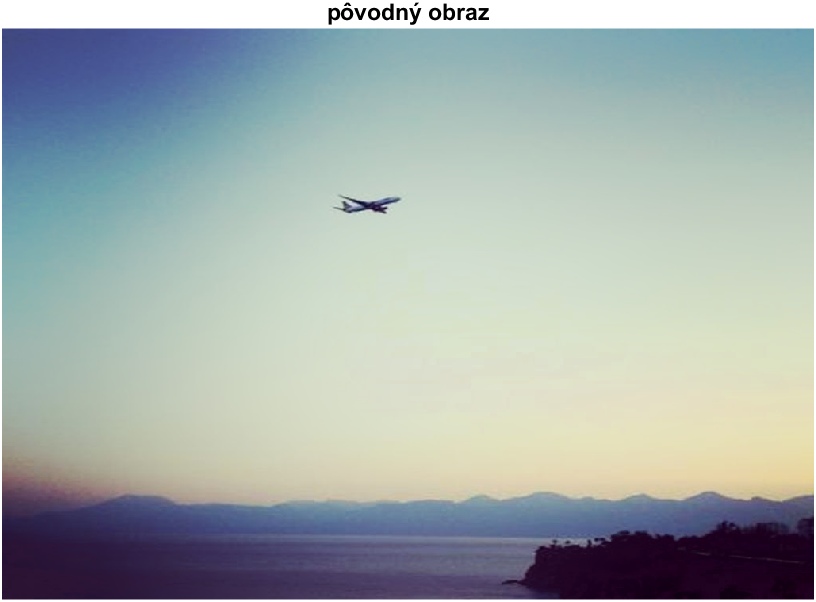
\includegraphics[width=.3\textwidth]{obrazky/canny/img.png}};
            \node (image2) [right of=image1] {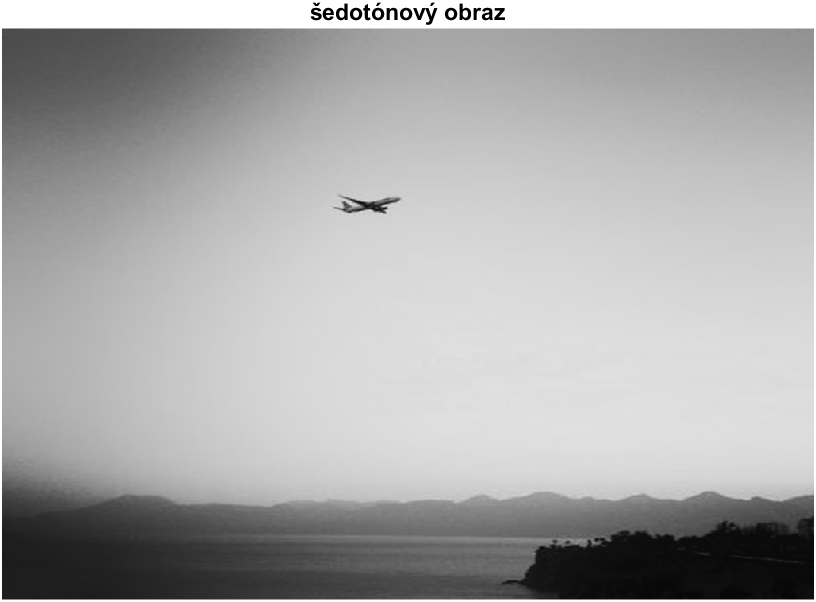
\includegraphics[width=.3\textwidth]{obrazky/canny/img_gray.png}};
            \node (image3) [right of=image2] {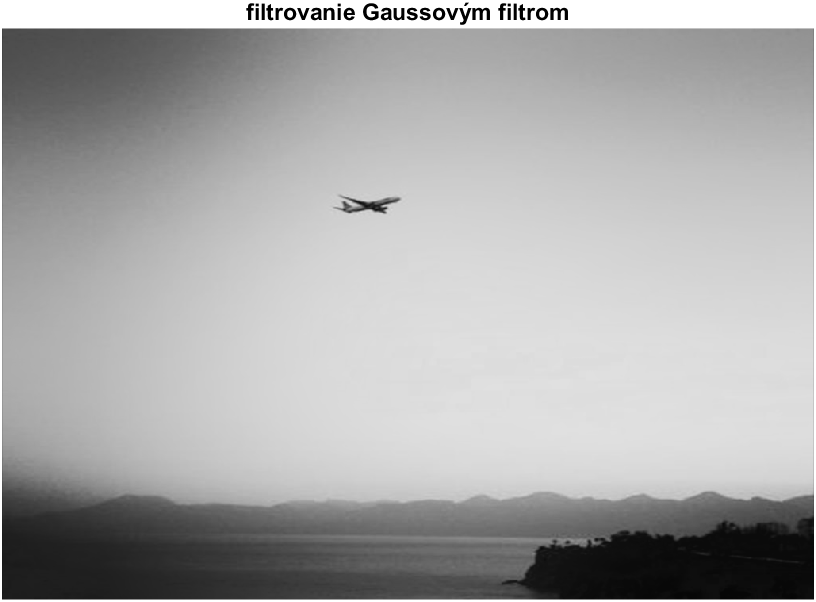
\includegraphics[width=.3\textwidth]{obrazky/canny/img_gauss.png}};
            \node (image4) [below of=image2] {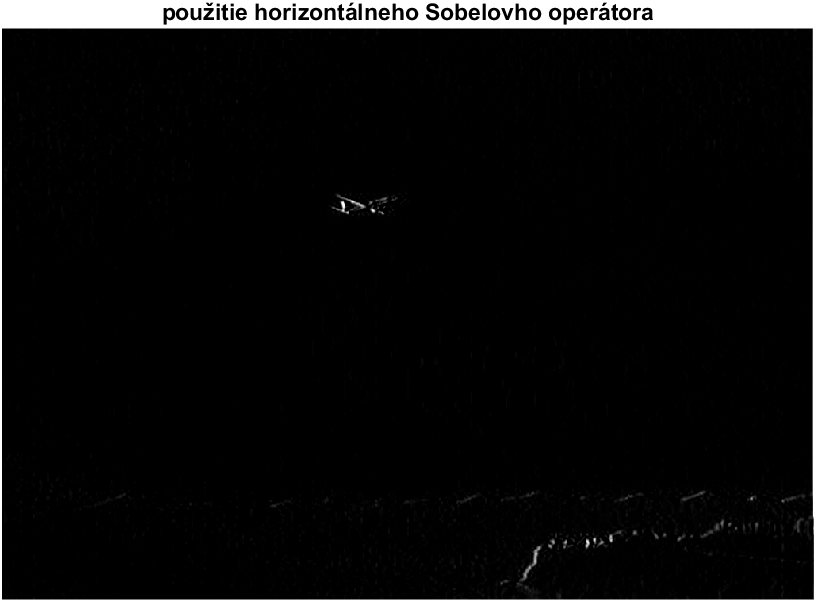
\includegraphics[width=.3\textwidth]{obrazky/canny/img_sobel_x.png}};
            \node (image5) [right of=image4] {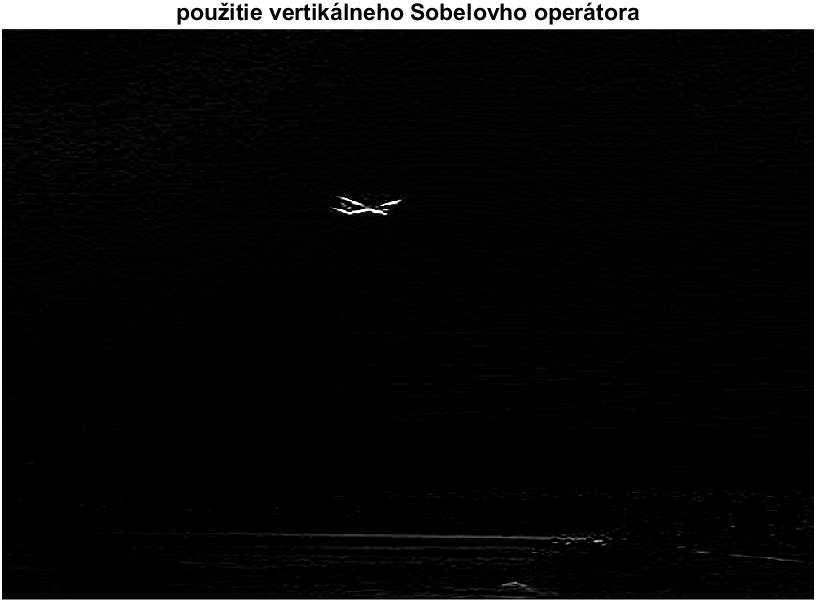
\includegraphics[width=.3\textwidth]{obrazky/canny/img_sobel_y.png}};
            \node (image6) [below of=image5] {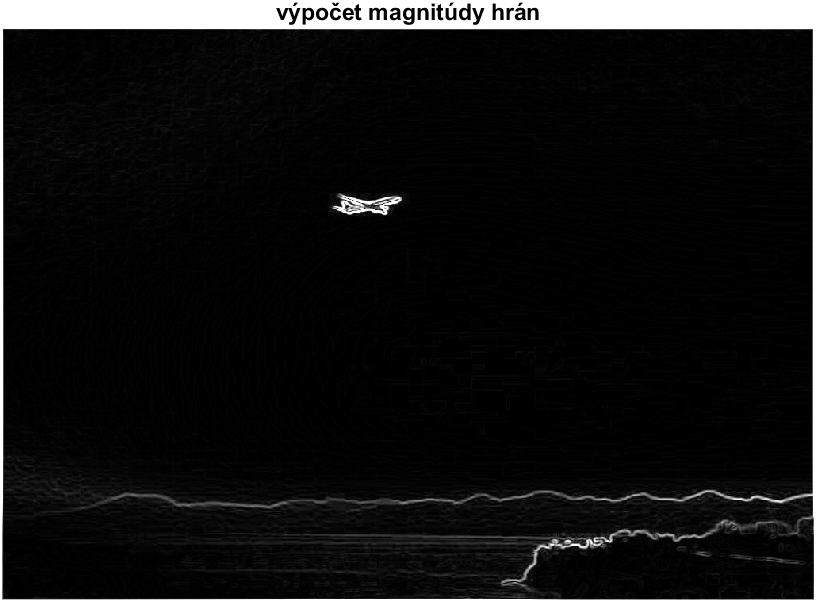
\includegraphics[width=.3\textwidth]{obrazky/canny/img_mag.png}};
            \node (image7) [left of=image6] {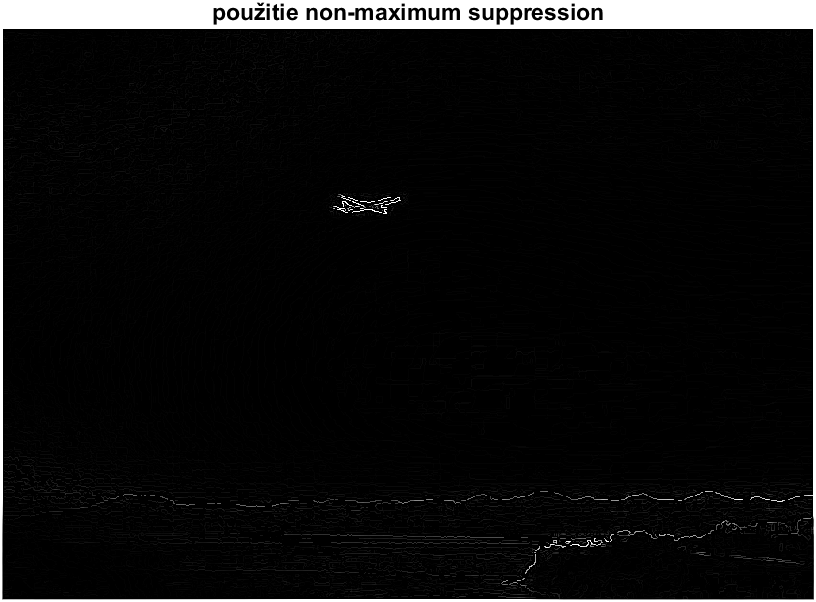
\includegraphics[width=.3\textwidth]{obrazky/canny/img_nms.png}};
            \node (image8) [left of=image7] {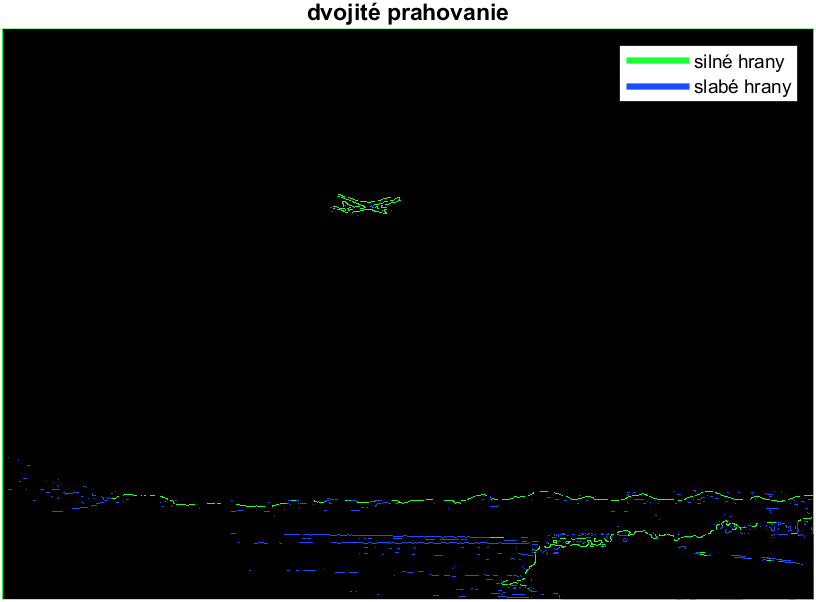
\includegraphics[width=.3\textwidth]{obrazky/canny/img_double_thresh.png}};
            \node (image9) [above of=image8] {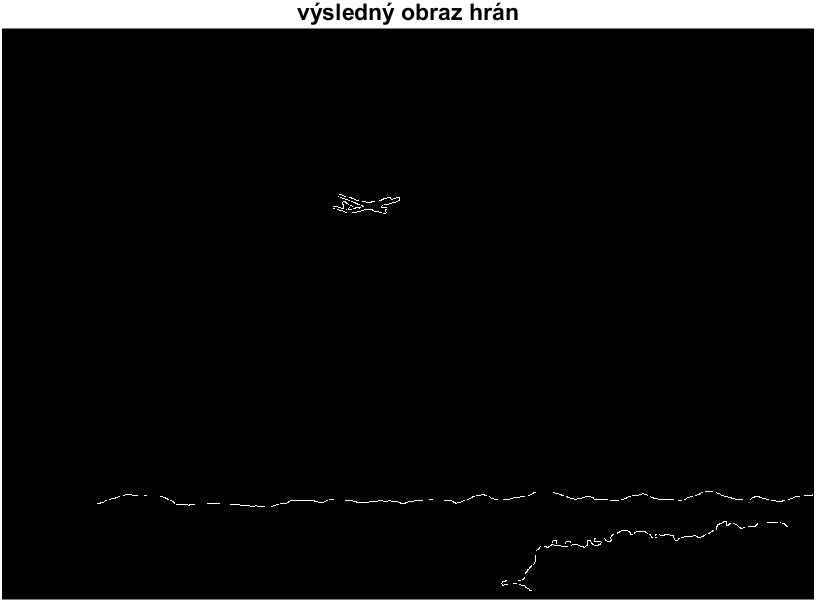
\includegraphics[width=.3\textwidth]{obrazky/canny/img_canny.png}};

            \draw[->] (image1) -- (image2) node[midway, above] {};
            \draw[->] (image2) -- (image3) node[midway, above] {};
            \draw[->] (image3) -- (image4) node[midway, above] {};
            \draw[->] (image3) -- (image5) node[midway, above] {};
            \draw[->] (image4) -- (image6) node[midway, above] {};
            \draw[->] (image5) -- (image6) node[midway, above] {};
            \draw[->] (image6) -- (image7) node[midway, above] {};
            \draw[->] (image7) -- (image8) node[midway, above] {};
            \draw[->] (image8) -- (image9) node[midway, above] {};
        \end{tikzpicture}
        \caption{Cannyho hranový detektor}
    \end{figure}

    Obraz hrán je možné ďalej spracovávať napríklad morfologickými operáciami: otvorením odstrániť krátke nevýznamné hrany, zatvorením spojiť hrany blízko pri sebe.

    Vyhľadávaním uzavretých kontúr v obraze hrán je možné identifikovať potenciálne objekty v obraze.

    \subsection{Detekcia horizontu pomocou Houghovej transformácie}

        Pokiaľ časť obrazu obsahuje horizont, je vhodnejšie detekovať lietajúce objekty len na~oblohe nad ním, aby sa predišlo falošným detekciám. Horizont je možné detekovať z~obrazu hrán pomocou Houghovej transformácie, podľa práce \cite{Janousek2018}. Vo výsledku Houghovej transformácie sa horizont prejaví ako najvýraznejšia čiara.


        \begin{figure}[H]
            \centering
            \begin{tikzpicture}[>=stealth, node distance=8cm]
                \node (image1) {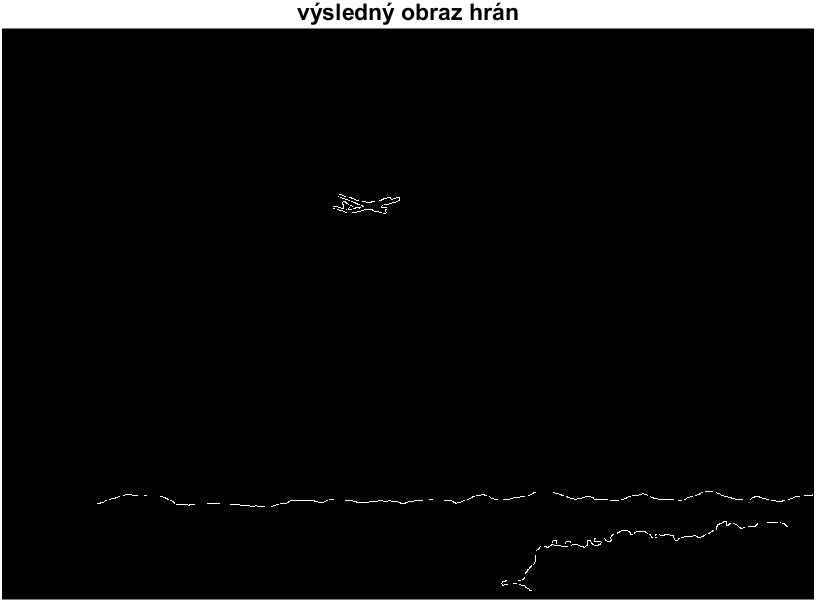
\includegraphics[width=.4\textwidth]{obrazky/canny/img_canny.png}};
                \node (image2) [below of=image1, yshift=2.5cm] {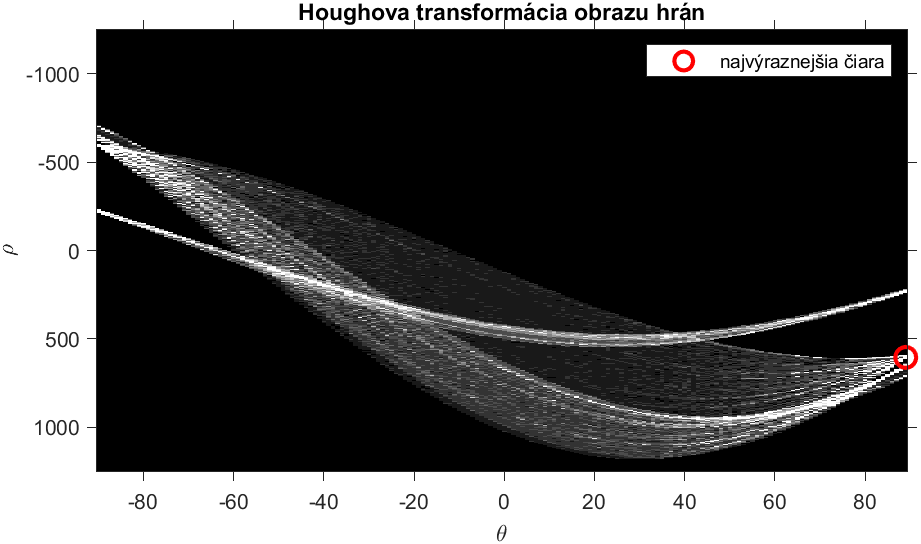
\includegraphics[width=.45\textwidth]{obrazky/canny/img_hough.png}};
                \node (image3) [right of=image2] {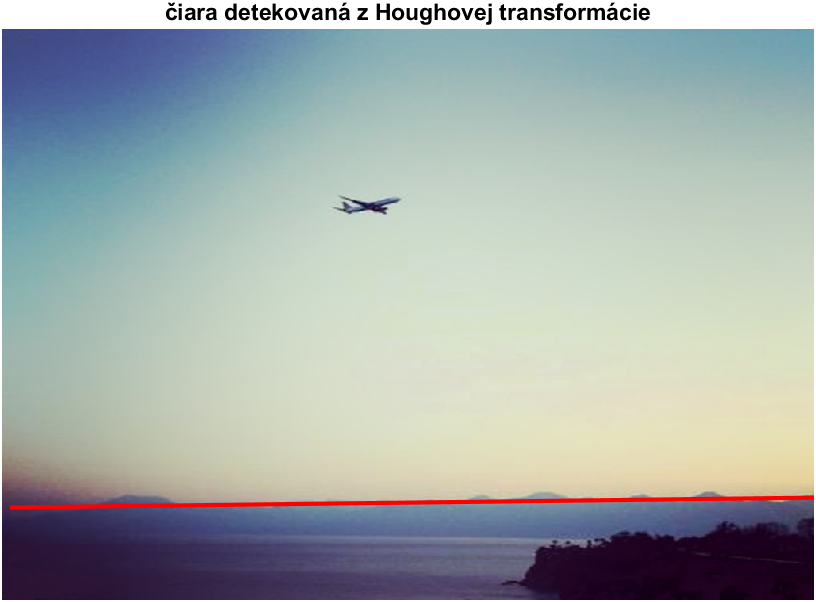
\includegraphics[width=.4\textwidth]{obrazky/canny/img_horizon.png}};

                \draw[->] (image1) -- (image2) node[midway, above] {};
                \draw[->] (image2) -- (image3) node[midway, above] {};
            \end{tikzpicture}
            \caption{Detekcia horizontu pomocou Houghovej transformácie}
        \end{figure}

    % \subsection{Detekcia objektov z kontúr}

\section{Detekcia pohybu}

    V prípade, že je požadovaná detekcia pohybujúcich sa objektov, je možnosťou detekovať ich práve podľa ich pohybu. Jednou z jednoduchých metód detekcie pohybu sú rozdielové metódy, pri ktorých je vypočítavaný rozdielový snímok z viacerých snímkov zo sekvencie $\{I_1, I_2, ..., I_n\}$. Rozdielový snímok môže byť:

    \begin{itemize}
        \item \textbf{jednostranný} - je najjednoduchší, nenesie informáciu o smere pohybu, vyhodnocuje sa len v miestach, kde $I_1(x,y) > I_2(x,y)$.
        \begin{equation}
            D(x,y) = \begin{cases}
                0 & I_1(x,y) - I_2(x,y) < \epsilon \\
                1 & I_1(x,y) - I_2(x,y) \geq \epsilon
            \end{cases}
        \end{equation}

        \item \textbf{obojstranný} - dostaneme ho upravením vzťahu pre jednostranný rozdielový snímok  použitím absolútnej hodnoty. Tým je dosiahnutá zameniteľnosť $I_1(x,y)$ a $I_2(x,y)$, vyhodnocuje sa teda na celom obraze. Neodstraňuje nedostatok informácie o smere pohybu, tá však nemusí byť nutnosťou.
        \begin{equation}
            D(x,y) = \begin{cases}
                0 & |I_1(x,y) - I_2(x,y)| < \epsilon \\
                1 & |I_1(x,y) - I_2(x,y)| \geq \epsilon
            \end{cases}
        \end{equation}

        \item \textbf{kumulovaný} - je vytvorený váženým súčtom jedno alebo obojstranných rozdielových snímkov. Je teda možné priemerovať pohyb za určitý čas určením každej váhy $\omega = \frac{1}{N-1}$ alebo určiť rôznym snímkom rôznu váhu a získať tak informáciu o smere pohybu.
        \begin{equation}
            D(x,y) = \sum_{i=1}^{N-1}\omega_i \cdot D_i(x,y)
        \end{equation}
    \end{itemize}

    Komplexnejšou metódou detekcie pohybu je vytvorenie rozdielového snímku nie medzi nasledujúcimi snímkami, ale aktuálnym snímkom a vytvoreným modelom pozadia. Ten je možné zostaviť:

    \begin{itemize}
        \item ako jeden obraz pozadia bez objektov,
        \item ako priemerný snímok niekoľkých snímkov pozadia,
        \item ako dynamický model - iteratívnym aktualizovaním podľa aktuálneho snímku. Tým sa model pozadia postupne prispôsobuje malým zmenám v prostredí.
    \end{itemize}

    Výpočet nového modelu pozadia $B_{i+1}(x,y)$ môže prebiehať napríklad pomocou lineárneho zabúdania, teda $B_{i+1}(x,y) = \alpha \cdot I_i(x,y) + (1 - \alpha) \cdot B_i(x,y)$.

    Obraz obsahujúci detekovaný pohyb je získaný rozdielom a prahovaním aktuálneho snímku a modelu pozadia. \cite{OpenCV2023}

    \begin{figure}[H]
        \centering
        \begin{tikzpicture}[node distance=.3cm, auto]

            % Define block styles
            \tikzstyle{block} = [rectangle, draw, fill=white!20, text width=12em, text centered, sharp corners, minimum height=4em]
            \tikzstyle{line} = [draw, -latex']

            % Nodes
            \node [block] (start) {prejdi na ďalší \\ snímok i \(\leftarrow\) i + 1};
            \node [block, below=of start] (calc_d1) {vypočítaj $D_1(x,y)$ medzi $I_i(x,y)$ a $I_{i-1}(x,y)$};
            \node [draw, diamond, aspect=4, below=of calc_d1] (check_d1) {vykazuje $D_1(x,y)$ významný pohyb?};
            \node [block, below=of check_d1] (calc_d2) {vypočítaj $D_2(x,y)$ medzi $I_i(x,y)$ a $B_i(x,y)$};
            \node [draw, diamond, aspect=4, below=of calc_d2] (check_d2) {vykazuje $D_2(x,y)$ významný pohyb?};
            \node [block, below=of check_d2] (calc_b) {vypočítaj $B_{i+1}(x,y)$};

            % Arrows
            \path [line] (start) -- (calc_d1);
            \path [line] (calc_d1) -- (check_d1);
            \path [line] (check_d1.west) -- ++(0,2.75) -- node [below = .3cm] {áno} (start.190);
            \path [line] (check_d1) -- node [near start] {nie} (calc_d2);
            \path [line] (calc_d2) -- (check_d2);
            \path [line] (check_d2.west) -- ++(-1,1) -- ++(0,7) -- node [near start] {áno} (start.170);
            \path [line] (check_d2) -- node [near start] {nie} (calc_b);
            \path [line] (calc_b.east) -- ++(3,1) -- ++(0,9) -- (start.east);

        \end{tikzpicture}
        \caption{Postup aktualizovania dynamického modelu pozadia}
    \end{figure}

    \begin{figure}[H]
        \centering
        \begin{tikzpicture} [node distance=1.5cm, auto]
            \node (image1) {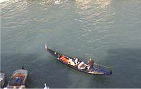
\includegraphics[width=.3\textwidth]{obrazky/motion/frame.png}};
            \node (space1) [below of=image1] {};
            \node (image2) [below of=space1] {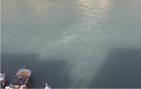
\includegraphics[width=.3\textwidth]{obrazky/motion/background.png}};
            \node (sum) [draw, rectangle, right of=space1, xshift=2.5cm] {D(x,y)};
            \node (threshold) [draw, rectangle, right of=sum, xshift=.5cm] {$\geq \epsilon$};
            \node (image3) [right of=threshold, xshift=2.5cm] {
\includegraphics[width=.3\textwidth]{obrazky/motion/motion.png}};

            \draw[->] (image1.east) to [out=0, in=90] (sum.north);
            \draw[->] (image2.east) to [out=0, in=270] (sum.south);
            \draw[->] (sum) -- (threshold);
            \draw[->] (threshold) -- (image3);
        \end{tikzpicture}
        \caption{Odčítanie pozadia}
    \end{figure}

\chapter{Popis objektov}

    Po nájdení objektov v obraze nasleduje ich popis pomocou príznakového vektoru. Ten predstavuje matematickú reprezentáciu segmentu obrazu vektorom o ľubovoľnom počte rozmerov. Jeho prvky popisujú farbu, textúru alebo tvar objektu. Samotný objekt nemusí byť rekonštruovateľný z jeho popisu, cieľom je podľa neho rozlíšiť od seba dva rôzne objekty.

    Vypočítané hodnoty príznakového vektoru majú niekoľko využití:

    \begin{itemize}
        \item \textbf{Párovanie objektov} v dvoch snímkoch, teda určenie, ktoré body alebo objekty v jednom snímku korelujú s tými v druhom snímku. Výhodou je to pri vyhľadávaní rovnakého objektu v po sebe nasledujúcich snímkoch pri sledovaní pohybu, či pri hľadaní rovnakého objektu v obraze z dvoch kamier.
        \item \textbf{Klasifikácia} objektov v obraze. Objekty rôznych tried majú často rôzne hodnoty určitých príznakov, je však nutné určiť, ktoré príznaky sú pre klasifikáciu relevantné.
    \end{itemize}

    \section{Popis tvaru}

        Jedny z najjednoduchších príznakov vychádzajú z tvaru objektu, používajú sa s~binárnym obrazom získaným napríklad prahovaním. \cite{Morse1998/2} Sú to napríklad:

        \begin{itemize}
            \item \textbf{Obsah} oblasti objektu, teda počet pixelov predstavujúcich objekt v binárnom obraze.
            \item \textbf{Obvod} je počet pixelov na hrane tvaru objektu. Diagonálne hrany môžu byť pri výpočte obvodu nadhodnotené v prípade, ak počítame s 4-okolím alebo podhodnotené, ak počítame s 8-okolím bodov na hrane. Je teda správnejšie počítať 1 pixel pre pravouhlé hrany a $\sqrt{2}$ pre diagonálne hrany.
            \item \textbf{Kompaktnosť} alebo kruhovosť je podobnosť tvaru ku kruhu. Vypočítava sa ako $\frac{Obvod^2}{Obsah}$ a je vždy vyššia alebo rovná kompaktnosti kruhu, čo je $4\pi$.
            \item \textbf{Excentricita} môže mať niekoľko definícií, jednou z nich je pomer dĺžky najdlhšej úsečky v tvare objektu s dĺžkou najdlhšej úsečky na ňu kolmej. Taktiež je to excentricita elipsy s rovnakým momentom druhého rádu, teda pomer vzdialeností ohnisiek a dĺžky hlavnej osy.
            \item \textbf{Pozdĺžnosť} je pomer výšky a šírky minimálneho opísaného obdĺžnika.
            \item \textbf{Pravouhlosť} alebo podobnosť s obdĺžnikom je pomer obsahu objektu a obsahu minimálneho opísaného obdĺžnika. Môže nadobúdať hodnoty do 1 a limitne môže klesať k 0.
            \item \textbf{Orientácia} alebo uhol hlavenj osi.
            \item \textbf{Eulerovo číslo} je topologický príznak značiaci rozdiel počtu spojených komponentov a dier v tvare objektu. Topológia popisuje vlastnosti tvaru, ktoré sa nemenia úpravami okrem delenia a spájania častí tvaru.
            \item \textbf{Počet konkávností} nie je topologickým príznakom, napriek jeho podobnosti s nimi. Získa sa spočítaním spojitých oblastí v rozdiele binárneho obrazu objektu a jeho konvexného obalu.
            \item \textbf{Konvexnosť} je možné určiť z pomeru obsahu objektu ku obsahu jej konvexného obalu.
        \end{itemize}

    \section{Fotometrické príznaky}

        Príznaky, ktorých hodnota závisí na jasových úrovniach popisovaného segmentu obrazu sa nazývajú fotometrické príznaky. Môže ísť o priemernú ($B_{priemer}$), minimálnu ($B_{min}$), maximálnu ($B_{max}$) hodnotu jasu objektu, rozdiel extrémov v objekte ($B_{dif.}$), priemerov jasu objektu $(\Omega)$ a pozadia $(\Phi)$ $(B_{dif. pozadia})$, či príznaky vyplývajúce z histogramu (H) alebo geometrických momentov.

        \begin{figure}[!ht]
            \centering
            \begin{minipage}[b]{0.45\textwidth}
                \[
                    B_{priemer} = \frac{1}{N} \cdot \sum_{(x,y) \in \Omega} f(x,y)
                \]
            \end{minipage}
            \begin{minipage}[b]{0.45\textwidth}
                \begin{equation}
                    B_{max} = max(f(x,y))
                \end{equation}
            \end{minipage}
            \begin{minipage}[b]{0.45\textwidth}
                \[
                    B_{dif. pozadia} = B_{priemer(\Omega)} - B_{priemer(\Phi)} 
                \]
            \end{minipage}
            \begin{minipage}[b]{0.45\textwidth}
                \[
                    B_{min} = min(f(x,y))
                \]
            \end{minipage}
            \begin{minipage}[b]{0.45\textwidth}
                \[
                    H_{priemer} = \frac{1}{N} \cdot \sum_{q=1}^{N} q \cdot h(q)
                \]
            \end{minipage}
            \begin{minipage}[b]{0.5\textwidth}
                \[
                    H_{kontrast} = \frac{1}{N} \cdot \sum_{q=1}^{N} (q \cdot h(q) - H_{priemer})^2
                \]
            \end{minipage}
            \begin{minipage}[b]{0.45\textwidth}
                \[
                    H_{energia} = \frac{1}{N} \cdot \sum_{q=1}^{N} h(q)^2
                \]
            \end{minipage}
            \begin{minipage}[b]{0.45\textwidth}
                \[
                    H_{entropia} = \frac{1}{N} \cdot \sum_{q=1}^{N} h(q) \cdot log_2h(q)
                \]
            \end{minipage}
        \end{figure}

        Z geometrických momentov, ktorých hodnoty sú závislé na afinných transformáciách (translácia, rotácia a úprava mierky) je možné úpravou získať príznaky na transformácii nezávislé. \cite{Erbo2017} Všeobecne je moment rádu (p,q) segmentu l(x,y) daný:
        \begin{figure}[!ht]
            \begin{minipage}[b]{0.45\textwidth}
                \[
                    m_{pq} = \int_{-\infty}^\infty\int_{-\infty}^\infty x^p y^q l(x,y) dx dy
                \]
                \centering
                (definícia)
            \end{minipage}
            \begin{minipage}[b]{0.45\textwidth}
                \begin{equation}
                    m_{pq} = \sum_{X}\sum_{Y} x^p y^q l(x,y)
                \end{equation}
                \centering
                (Pre konečný diskrétny obraz)
            \end{minipage}
        \end{figure}

        Centralizované momenty $\mu_{pq}$, vztiahnuté k ťažisku objektu $(x_t,y_t) = (\frac{m_{10}}{m_{00}},\frac{m_{01}}{m_{00}})$, získavajú nezávislosť na transláciu:
        \begin{equation}\mu_{pq} = \sum_X\sum_Y\ (x-x_t)^p \cdot (y-y_t)^q \cdot l(x,y)\end{equation}

        Z centralizovaných momentov je možné určiť momentové invarianty, základných sedem je nazývaných Huovými momentami.

\chapter{Klasifikácia}

    Ďalším krokom je zaradenie detekovaných objektov do tried, teda ich klasifikácia. Klasifikácia objektov vychádza z ich popisu.

    \section{Klasifikátory}

        Klasifikátory sú algoritmy schopné automaticky kategorizovať dáta do dvoch a viac tried. Modely určené na~klasifikáciu sú väčšinou učené s učiteľom, je potrebné pomerne veľké množstvo anotovaných dát. Výsledkom je schopnosť generalizovať klasifikáciu na nových neznámych dátach.

        Existuje niekoľko typov klasifikátorov, napríklad \textbf{Lineárne klasifikátory} rozdeľujú príznakový priestor nadrovinami, \textbf{Bayesov klasifikátor} vypočítava pravdepodobnosť zaradenia do triedy. Ako klasifikátor môžu slúžiť aj plne prepojené \textbf{neurónové siete}.

    \section{Konvolučné neurónové siete}

        Na rozdiel od plne prepojenej neurónovej siete, sú \ac{CNN} prispôsobené na prácu s obrazom ako so vstupným signálom. Pracujú na princípe výpočtu príznakov pomocou konvolučnej časti siete a klasifikáciou plne prepojenou sieťou. Ich architektúra je usporiadaná do vrstiev, štandardne po sebe nasledujú:

        \begin{enumerate}
            \item \textbf{Konvolučná vrstva} - používa konvolučné filtre na extrakciu príznakov z obrazu.
            \item \textbf{Aktivačná vrstva} - aplikuje aktivačnú funkciu, často napríklad \ac{ReLU} na každý bod. Zavádza do siete nelinearitu a pomáha zachytávať zložitejšie vzory.
            \item \textbf{Pooling vrstva} - redukuje priestorové rozlíšenie vstupných dát. Tým sa zníži výpočtová náročnosť nasledujúcich vrstiev. Najčastejšie sa používa \emph{max pooling}, teda výber najvyššej hodnoty v okolí.
        \end{enumerate}

        Väčšinou je použitá kombinácia niekoľko \textbf{konvolučných} vrstiev nasledovaných \textbf{aktivačnou} vrstvou, po ktorých \textbf{pooling} vrstva pripraví redukovaný vstup pre ďalšie vrstvy. Takýchto kombinácii nasleduje niekoľko, posledná je pripojená na plne prepojenú neurónovú sieť. Konvolučná časť slúži na vyhľadávanie príznakov, plne prepojená časť na klasifikáciu pomocou nich.

        \begin{figure}[h]
            \centering
            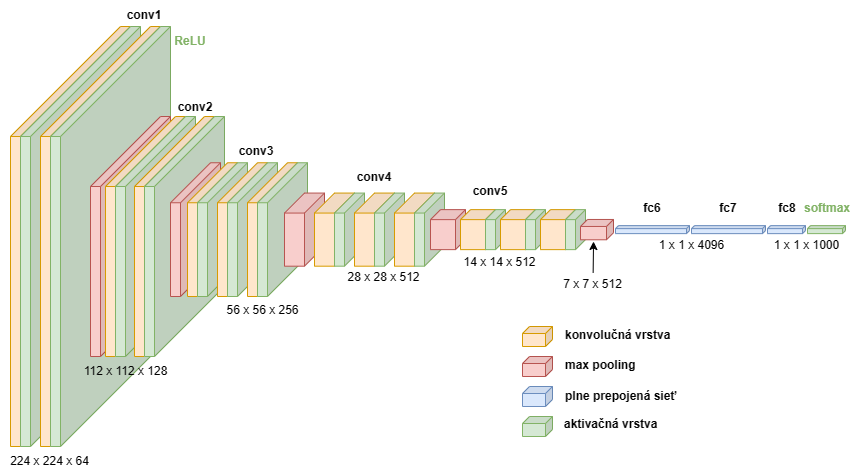
\includegraphics[width=.9\textwidth]{obrazky/cnn/cnn.png}
            \caption{Príklad architektúry konvolučnej neurónovej siete}
        \end{figure}

        Rozmery vrstiev závisia na tvare vstupného signálu. V prípade šedotónového obrazu je každý bod obrazu reprezentovaný jednou skalárnou hodnotou, v prípade farebného obrazu záleží počet hodnôt na pixel na farebnom modeli. Klasifikáciou z farebného obrazu získavame väčšie množstvo informácii, ale je vyžadovaný vyšší výkon, nakoľko sa konvolučné filtre aplikujú po jednom na každú zložku obrazu (teda v prípade RGB modelu na červenú, zelenú a modrú zložku samostatne).

        Výstup z poslednej vrstvy plne prepojenej časti siete je výstupom z celej \ac{CNN}. Výstupy klasifikačnej neurónovej siete s úlohou klasifikovať viacero tried mávajú formáty:

        \begin{itemize}
            \item Jeden výstup, ktorého hodnota určuje triedu, do ktorej sú vstupné dáta sieťou priradené.
            \item Vektor výstupov s toľkými hodnotami, na koľko tried je naučená sieť klasifikovať. Hodnoty výstupov môžu reprezentovať:
            \begin{itemize}
                \item Ohodnotenie triedy (score-based classification). V tomto prípade čísla na výstupe nemajú samostatne význam, ale ako predpoveď je určená trieda s najvyšším skóre.
                \item Pravdepodobnosť zaradenia do danej triedy. Tá je získaná použitím výstupnej aktivačnej vrstvy typu \emph{softmax}, ktorá spôsobí, že každý z výstupov má hodnotu od 0 do 1 a súčet všetkých výstupov je 1.
            \end{itemize}
        \end{itemize}

\chapter{Detekcia a klasifikácia v jednom kroku}
    Existuje niekoľko metód schopných detekcie aj~klasifikácie pomocou jediného modelu. Vďaka tomu je možné vynechať krok detekcie a~získať priamo klasifikované orámovania, čím sa~systém detekcie zjednoduší. Je však nutné porovnať výkon a~kvalitu detekcie a~klasifikácie v~jednom kroku s~prístupom so~samostatnou detekciou a~klasifikáciou.

    \section{R-CNN}

        \ac{R-CNN} sú skupina modelov strojového učenia zaločená na \ac{CNN}. Ich cieľom je nájdenie a~klasifikovanie objektov v obraze. Ich výstupom je množina rámčekov ohraničujúcich objekty a im pridelené triedy.

        \ac{R-CNN} pracujú v niekoľkých etapách:
        \begin{enumerate}
            \item \textbf{Selektívne vyhľadávanie} - vstupný obraz je spracovaný a sú extrahované \ac{RoI}, teda orámované oblasti obrazu, ktoré by mohli obsahovať objekty alebo ich časti. Počet takto navrhovaných oblastí môže dosahovať niekoľko tisíc.
            \item \textbf{Extrakcia príznakov} - každý \ac{RoI} je predložený ako vstup pre naučenú \ac{CNN}, ktorá vyprodukuje príznakový vektor pre každý \ac{RoI}.
            \item \textbf{Klasifikácia} - pomocou skupiny modelov \ac{SVM} je podľa príznakov extrahovaných \ac{CNN}, klasifikovaný každý \ac{RoI} do jednej z určených tried alebo ako pozadie - teda nepatriaci do žiadnej triedy.
            \item \textbf{Regresia ohraničení} - konečný krok, zvyšujúci presnosť orámovania objektov. Používa sa pri ňom naučený model nezávislý na mierke nazývaný \emph{bounding box regressor}. Jeho výstup je štvorrozmerný, skladá sa z polohy a rozmerov ohraničujúceho obdĺžnika.
        \end{enumerate}

        \ac{R-CNN} sú efektívne, no náročné na výpočtový výkon. Z toho dôvodu boli vyvinuté rýchlejšie varianty \emph{Fast R-CNN} a \emph{Faster R-CNN}.

        \emph{Fast R-CNN} aplikuje \ac{CNN} na celý vstupný obraz a extrahuje z neho mapu príznakov. Až na výslednú mapu aplikuje takzvaný \ac{RoI} \emph{pooling}, ktorý extrahuje príznaky pre každý \ac{RoI}, pomocou okna pevnej veľkosti. Zvyšok modelu pracuje podobne ako \ac{R-CNN} s využitím plne prepojenej siete na klasifikáciu a generovanie orámovaní.

        \emph{Faster R-CNN} nadväzuje na \emph{Fast R-CNN} nahradením selektívneho vyhľadávania modelom typu \ac{RPN}. Vstupný obraz prechádza predučenou \ac{CNN}, sú extrahované príznaky. \ac{RPN} využije nájdené príznaky, aby určila, kde sa nachádzajú potenciálne objekty v obraze. V konečnom kroku sú klasifikované navrhnuté ohraničené oblasti podľa príznakov extrahovaných v predošlom kroku. \emph{Faster R-CNN} je dostatočne rýchla na použitie v reálnom čase.

    \section{YOLO}
        \ac{YOLO} je populárny algoritmus detekcie, ktorý na rozdiel od \ac{R-CNN} rozdeľuje obraz do mriežky a postupne aplikuje klasifikátor, eliminujúc krok návrhu regiónov záujmu. Zameriava sa teda na rýchlosť a jednoduchosť. Postupuje nasledovne:

        \begin{enumerate}
            \item Vstupný obraz je rozdelený na mriežku $S \times S$, ktorej veľkosť závisí na verzii \ac{YOLO}.
            \item V každej bunke mriežky je predikovaný určitý počet ohraničených oblastí a im priradené skóre dôveryhodnosti. Tie značia úroveň istoty, že oblasť obsahuje objekt a že dané ohraničenie je správne. Oblasti sú popísané štyrmi číslami, dve súradnice stredného bodu oblasti a dva rozmery ohraničujúceho obdĺžnika.
            \item Je použitých viacero klasifikátorov. Počas trénovania je jednému z prediktorov udelená zodpovednosť za~predikovanie daného objektu podľa toho, ktorý z nich dosahuje najväčší \ac{IoU}. Výstupom klasifikácie v \ac{YOLO} je vektor predikcii pravdepodobností, že objekt obsiahnutý v danom ohraničení patrí do každej triedy. Celkový výstup YOLOv8 je tenzor obsahujúci zoznam všetkých klasifikovaných oblastí.
            \item Každá bunka predikuje rozdelenie pravdepodobnosti všetkých tried.
        \end{enumerate}

        Hlavnou výhodou \ac{YOLO} je rýchlosť. Všeobecne pracuje rýchlejšie a s menším požadovaným výpočtovým výkonom. Na druhú stranu má nevýhody spôsobené obmedzením veľkosti orámovaných oblastí. Presnosť \ac{YOLO} býva nižšia pri primalých objektoch, pre použitia vyžadujúce vyššiu presnosť sa môže javiť ako výhodnejšie použiť iné modely.

        \subsection{Non-Maximum Suppression}
            Výstup zo siete YOLOv8 je vo formáte zoznamu 8400 potenciálnych orámovaní, ktoré sú tvorené súradnicami stredového bodu, rozmermi orámovania a ohodnotením dôveryhodnosti, že orámovanie obsahuje objekt pre každú triedu. Typickým problémom detekčných modelov je že ich výstup obsahuje niekoľko prekrývajúcich sa orámovaní patriacich rovnakému objektu. Algoritmus \ac{NMS} pre odstránenie redundantných orámovaní postupuje podobne ako pri jeho aplikovaní na obraz hrán. Výsledkom je nájdenie najlepšieho orámovania pre každý objekt v obraze. Pred jeho použitím je nutné určiť dva parametre. Prvým je prah \ac{IoU} medzi orámovaniami $\tau$, druhým prah dôveryhodnosti $T$. \ac{NMS} začne prácu s množinou orámovaní $B$ ohodnotených úrovňou dôveryhodnosti $S$.

            \begin{figure}[H]
                \centering
                \begin{tikzpicture} [node distance=7cm, auto]
                    \tikzstyle{line} = [draw, -latex']
                    \node (image1) {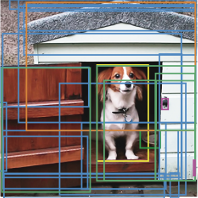
\includegraphics[width=.3\textwidth]{obrazky/nms/before.png}};
                    \node (image2) [right of=image1] {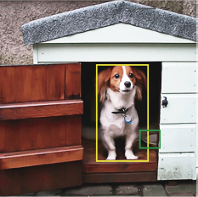
\includegraphics[width=.3\textwidth]{obrazky/nms/after.png}};
                    \path [line] (image1) -- (image2);
                \end{tikzpicture}
                \caption{Vstup a výsledok \ac{NMS}}
            \end{figure}

            \begin{figure}[H]
                \centering
                \begin{tikzpicture}[node distance=.3cm, auto]

                    % Define block styles
                    \tikzstyle{block} = [rectangle, draw, fill=white!20, text width=18em, text centered, sharp corners, minimum height=4em]
                    \tikzstyle{line} = [draw, -latex']

                    % Nodes
                    \node [draw, rectangle] (start) {začiatok};
                    \node [block, below=of start] (prepare) {Priprav prázdnu množinu výsledných filtrovaných orámovaní $F = \emptyset$};

                    \node [block, below=of prepare] (filter_conf) {Z množiny orámovaní $B$ odstráň orámovania s prinízkou dôveryhodnosťou
                    \\$B \leftarrow \{b \in B | S(b) \geq T\}$
                    };

                    \node [block, below=of filter_conf] (order_conf) {Zoraď orámovania ostávajúce v množine $B$};

                    \node [draw, diamond, aspect=4, below=of order_conf] (check_remaining) {\parbox{15em}{\centering Obsahuje $B$ ešte orámovania? \\$B \neq \emptyset$}};

                    \node [block, below=of check_remaining] (select_b) {Vyber prvé orámovanie $b$ z množiny $B$ s najvyššou dôveryhodnosťou $S(b)$};

                    \node [block, below=of select_b] (add_b) {Vlož $b$ do množiny $F$ a odober ho z množiny $B$:
                    \\$F \leftarrow F  \bigcup  \{b\}$ 
                    \\$B \leftarrow B - \{b\}$};

                    \node [draw, diamond, aspect=4, below=of add_b] (check_iteration) {\parbox{15em}{\centering Boli skontrolované všetky \\zostávajúce orámovania $r$ v $B$?}};

                    \node [draw, diamond, aspect=4, below=of check_iteration] (check_iou) {\parbox{15em}{\centering Patrí toto ohraničenie rovnakému objektu poďla IoU? \\$IoU(b,r) \geq \tau$}};

                    \node [block, below=of check_iou] (remove_r) {Odober $r$ z množiny $B$:
                    \\$B \leftarrow B - \{b\}$};

                    \node [draw, rectangle, right=of select_b] (end) {koniec};

                    % Arrows
                    \path [line] (start) -- (prepare);
                    \path [line] (prepare) -- (filter_conf);
                    \path [line] (filter_conf) -- (order_conf);
                    \path [line] (order_conf) -- (check_remaining);
                    \path [line] (check_remaining) -- node [near start] {áno} (select_b);
                    \path [line] (check_remaining.350) -- node [near start] {nie} (end);
                    \path [line] (select_b) -- (add_b);
                    \path [line] (add_b) -- (check_iteration);
                    \path [line] (check_iteration) -- node [near start] {nie} (check_iou);
                    \path [line] (check_iteration.175) -- node [near start] {áno} (check_remaining.185);
                    \path [line] (check_iou) -- node [near start] {áno} (remove_r);
                    \path [line] (check_iou.165) -- node [near start] {nie} (check_iteration.190);
                    \path [line] (remove_r.0) -- ++(3.5,0) -- ++(0,4) -- (check_iteration.0);
                \end{tikzpicture}
                \caption{Algoritmus Non-Maximum Suppression pre orámovanie objektov}
            \end{figure}

\chapter{Ukladanie naučených modelov}
    Neurónové siete využívané v tejto práci je nutné po ich naučení uložiť tak, aby ich dokázala aplikácia systému v zariadení načítať a použiť. K tomu je dostupných niekoľko rôznych formátov.

    \section{ONNX}
        ONNX je otvorený formát vybudovaný na reprezentáciu rôznych modelov strojového učenia. Definuje stavebné bloky modelov strojového a hlbokého učenia so spoločným formátom súborov dovoľúcim vývojárom používať uložený model s rôznymi nástrojmi a programami. Hlavnou výhodou je interoperabilita umožňujúca vytváranie modelov, ich testovanie a používanie v nezávislých aplikáciách. Ak je pre aplikáciu známy formát vstupu a výstupu, sú modely uložené v ONNX rovnocenné z hľadiska ich ovládania, vďaka čomu je implementácia využitia modelov rovnakého druhu zjednodušená.

    \section{Keras}
        Knižnica \emph{Keras} patriaca pod knižnicu \emph{Tensorflow} umožňujúca prácu so strojovým učením je jednou s často používaných knižníc pre \emph{Python} s týmto zameraním. Je v nej implementovaný vlastný formát súborov na ukladanie modelov, z ktorých je možné jednoducho načítať model postavený z komponentov z knižnice \emph{Keras}. Vďaka existencii špecializovaných verzii knižníc \emph{Tensorflow} na využitie s procesorom aj GPU je možné nainštalovaním správnej verzie knižnice rozhodnúť o využití výpočtového výkonu počítača.

\chapter{Vyhodnotenie kvality detekcie}
    K porovnaniu a vyhodnoteniu kvality výsledkov rôznych prístupov je nutné zhotoviť anotovaný dataset so snímkami zachytenými za reálnych podmienok kamerou priamo na zariadení. Použitím porovnávaných prístupov na snímky v tomto datasete a ich následným porovnaním s anotáciou je možné vypočítať metriky popisujúce ich kvalitu detekcie a klasifikácie.

    \section{Kvalita orámovania}
        Často používanou metrikou presnosti orámovania je takzvané \ac{IoU}. To je získané porovnaním orámovania určeného pri anotácii a orámovania predikovaného detektorom.

        \begin{figure}[h]
            \centering
            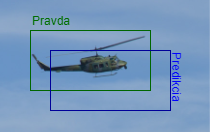
\includegraphics[width=.6\textwidth]{obrazky/metrics/detection.drawio.png}
            \caption{Orámovanie na anotovanom snímku}
        \end{figure}

        Pred výpočtom je nutné určiť obsah prieniku a následne zjednotenia obdĺžnikov anotovaného a predikovaného orámovania. Zvolíme súradnicový systém s počiatkom v ľavom hornom rohu so súradnicami stúpajúcimi smerom dolu a doprava. Prienik dvoch obdĺžnikov je možné určiť nájdením ľavého horného rohu, zvolením najvyšších súradníc ľavých horných rohov obidvoch obdĺžnikov. Pravý dolný roh je naopak nájdený ako najnižšie súradnice pravých dolných rohov. Obsah prieniku je potom súčtom obsahov obdĺžnikov po odčítaní obsahu ich prieniku.

        \begin{figure}[h]
            \centering
            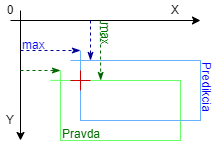
\includegraphics[width=.4\textwidth]{obrazky/metrics/find intersection.drawio.png}
            \caption{Nájdenie prvého bodu prieniku orámovaní}
        \end{figure}

        \begin{equation}
            IoU = \frac{Obsah(B_{pravda} \bigcap B_{predikcia})}{Obsah(B_{pravda} \bigcup B_{predikcia})} = \frac{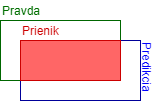
\includegraphics[height=3cm]{obrazky/metrics/intersection.drawio.png}}{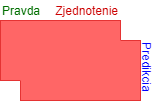
\includegraphics[height=3cm]{obrazky/metrics/union.drawio.png}}
        \end{equation}

        Hodnota \ac{IoU} sa~pohybuje medzi 0~a~1, pričom vyššia hodnota značí vyššiu presnosť. Hodnota 1 znamená dokonalé prekrytie.

    \section{Kvalita klasifikácie}
        \subsection{Matica zámien}
            Matica zámien (confusion matrix) je prehľadné zobrazenie výsledkov klasifikácie určitej množiny objektov. Vykresľuje sa~ako~tabuľka rozdeľujúca počet vzoriek z~každej skutočnej triedy podľa ich~predikovanej triedy. Ak~sú skutočné a~predikované triedy v~tabuľke v~rovnakom poradí, na~diagonále sa~nachádzajú počty správne zaradených, mimo diagonály zas~nesprávne zaradených inštancií.

        \subsection{Metriky vychádzajúce z matice zámien}
            Elementy matice zámien je možné roztriediť podľa správnosti ich klasifikácie do konkrétnej triedy. Hodnoty metrík klasifikácie sú vypočítavané vzhľadom na konkrétnu triedu alebo pre celkovú klasifikáciu.

            Riadky matice \ref{fig:example_confusion_matrix} reprezentujú skutočnosť, stĺpce predikciu. P (pozitívne) zaradenie reprezentuje prvky zaradené do triedy, pre ktorú chceme počítať metriky klasifikácie. N (negatívne) značí ostatné triedy.

            \begin{figure}[!h]
                \begin{minipage}[b]{0.38\textwidth}
                    \begin{tabular}{c|c|c|c|}
                          & N  &  P & N  \\
                        \hline
                        N & TN & FP & TN \\
                        \hline
                        P & FN & TP & FN \\
                        \hline
                        N & TN & FP & TN \\
                        \hline
                    \end{tabular}
                    \centering
                    \caption{Rozdelenie prvkov matice}
                    \label{fig:example_confusion_matrix}
                \end{minipage}
                \begin{minipage}[b]{0.6\textwidth}
                    \begin{itemize}
                        \item \textbf{TP} (true positive) sú inštancie zaradené správne do triedy, ktorej klasifikáciu chceme ohodnotiť.
                        \item \textbf{TN} (true negative) sú zaradené správne do iných tried.
                        \item \textbf{FP} (false positive) sú inštancie nesprávne označené za sledovanú triedu.
                        \item \textbf{FN} (false negative) sú naopak označené ako sledovaná trieda, no správne patria do jednej z ostatných tried.
                    \end{itemize}
                \end{minipage}
            \end{figure}

            \begin{itemize}
                \item \textbf{Presnosť (precision)} vyjadruje ako často, keď model predpovedá určitú triedu, je jeho predpoveď správna.
                \begin{equation}
                    Precision = \frac{TP}{TP + FP}
                \end{equation}
                \item \textbf{Úplnosť (recall)} značí ako často model správne vyhodnotí objekt ako patriaci do danej triedy v pomere ku skutočnému počtu objektov z tej triedy. Nízke skóre úplnosti značí že model primálo často predpovedá danú triedu.
                \begin{equation}
                    Recall = \frac{TP}{TP + FN}
                \end{equation}
                \item \textbf{F1 skóre} je kombináciou presnosti a úplnosti. Využíva sa v prípade hľadania rovnováhy medzi presnosťou a úplnosťou.
                \begin{equation}
                    F1 = \frac{2 \times Precision \times Recall}{Precision + Recall}
                \end{equation}
                \item \textbf{Správnosť (accuracy)} je pomer spočtu právne klasifikovaných inštancii ku počtu všetkých inštancii.
                \begin{equation}
                    Accuracy = \frac{TP + TN}{P + N}
                \end{equation}
                \item \textbf{Citlivosť (sensitivity)} znamená, ako často model správne vyhodnocuje objekty danej triedy ako patriace do tej triedy.
                \begin{equation}
                    Sensitivity = \frac{TP}{P}
                \end{equation}
                \item \textbf{Špecificita (specificity)} na druhú stranu vyjadruje, ako často sú správne vyhodnotené prvky nepatriace do danej triedy.
                \begin{equation}
                    Specificity = \frac{TN}{N}
                \end{equation}
            \end{itemize}

    \section{Výkon detekcie}
        \subsection{Snímková frekvencia}
            Dôležitým parametrom systému detekcie je frekvencia, s akou je schopný získavať a spracovávať snímky. V prípade, že je snímková frekvencia príliš nízka, je možné, že príliš rýchlo sa pohybujúce objekty nestrávia v zábere kamery dostatočný čas na to, aby boli zachytené na aspoňi jednom snímku. Jedny z hlavných faktorov obmedzujúcich snímkovú frekvenciu sú:
            \begin{itemize}
                \item Maximálna snímkovacia frekvencia kamery pri danom rozlíšení.
                \item Výpočtový výkon zariadenia, na ktorom je systém spustený.
                \item Zložitosť metód použitých v systéme.
            \end{itemize}

        \subsection{Oneskorenie}
            V rôznych oblastiach využitia systému detekcie môže byť požadované spracovanie vstupného obrazu v určitom časovom úseku. Ak je potrebné dosiahnuť čo najnižšie oneskorenie, musia byť zvolené dostatočne jednoduché metódy s prihliadnutím na výkon zariadenia.

        \begin{figure}[!ht]
            \begin{center}
                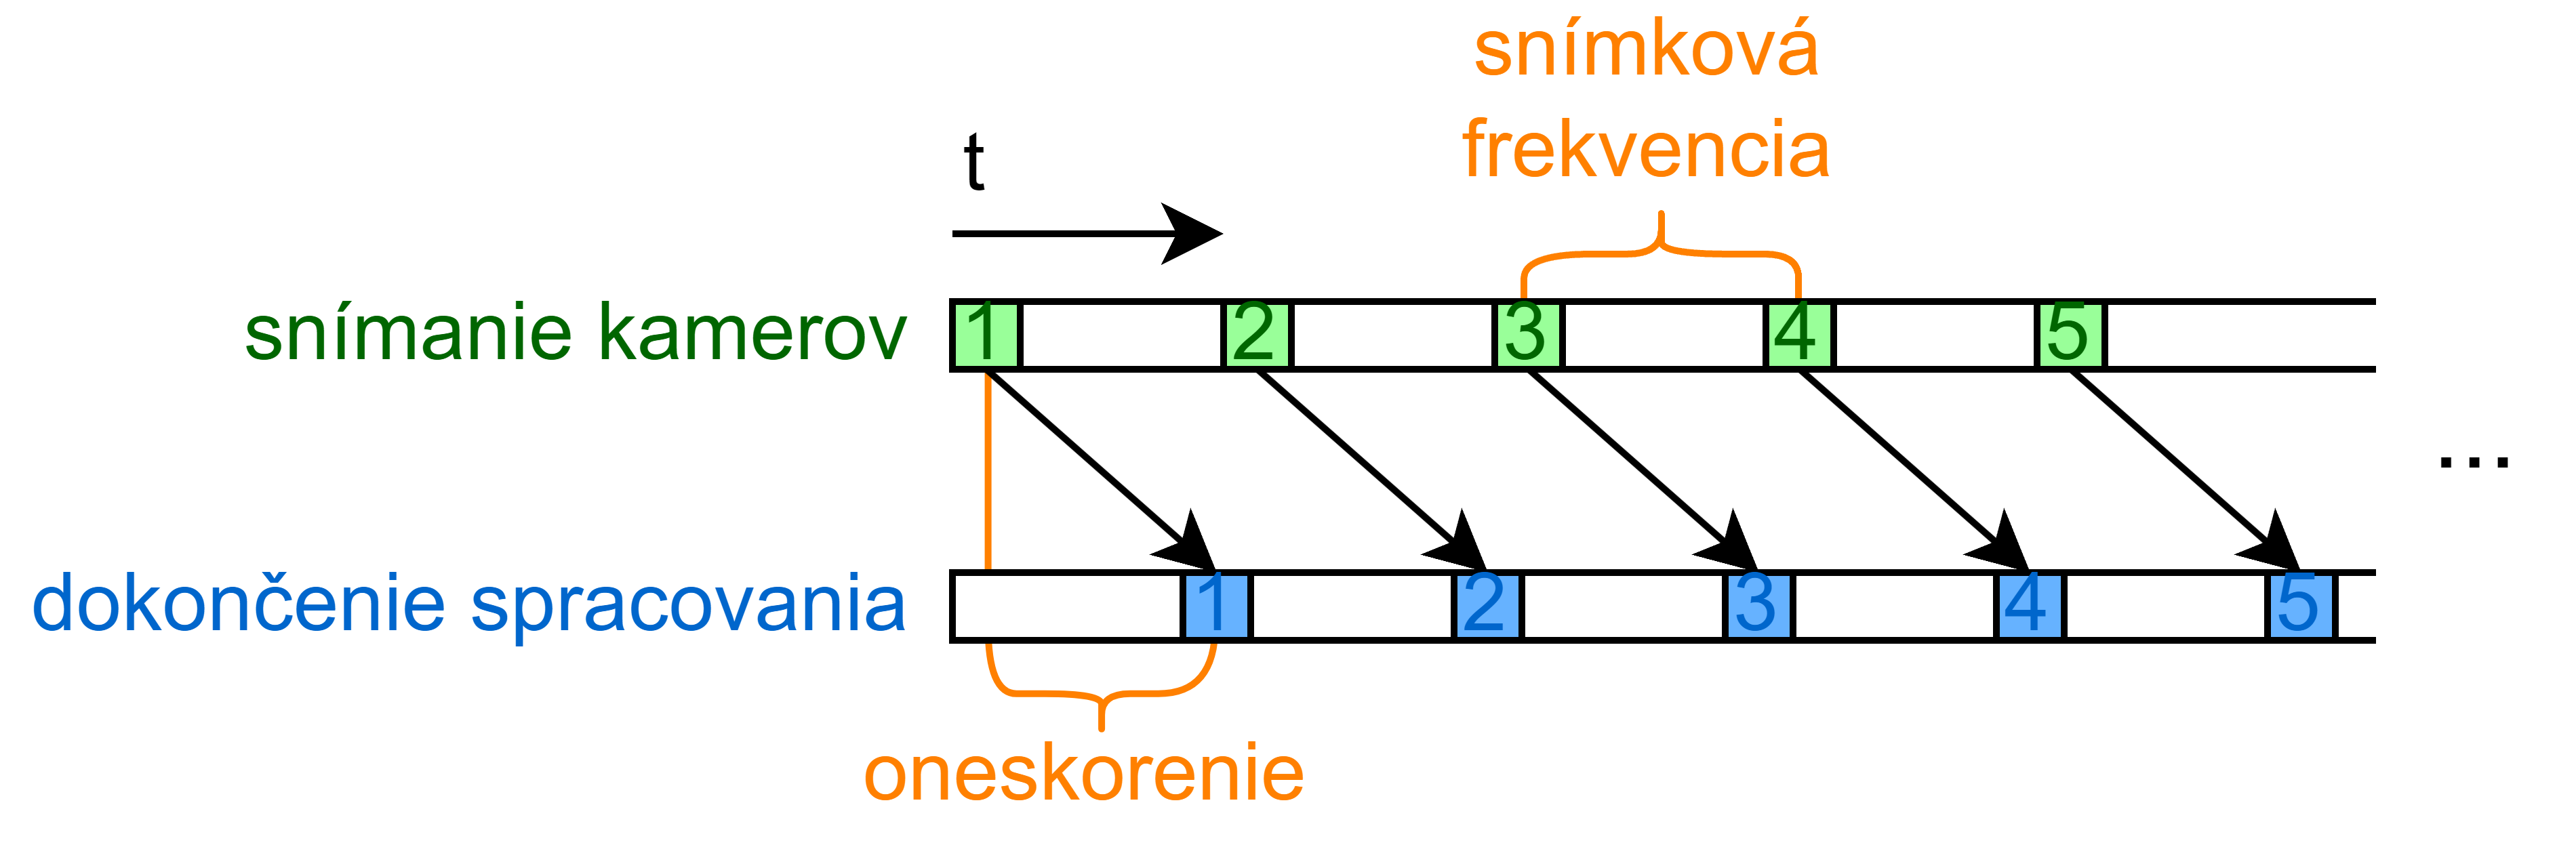
\includegraphics[width=.8\textwidth]{obrazky/metrics/fps_latency.drawio.png}
            \end{center}
            \caption{Snímková frekvencia a oneskorenie}
        \end{figure}

\chapter{Návrh usporiadania hardvérových komponentov}

    Táto kapitola sa zameriava na návrh a implementáciu prenosného zariadenia pre~detekciu, klasifikáciu a trasovanie lietajúcich objektov. Cieľom návrhu je vytvorenie zariadenia s možnosťou nasadenia v čo najrôznejších podmienkach. Jednou z podmienok je teda jeho prenosnosť, možnosť napájania z akumulátora a nezávislosť na~iných zariadeniach pri jeho nastavení a používaní.

    \section{Jednodoskový počítač}
    
        Jedným z najčastejšie používaných jednodoskových počítačov je rada \emph{Raspberry Pi}. V čase návrhu bol najnovším model \emph{Pi 4 model B}. Tento model disponuje:
        \begin{itemize}
            \item 1.5GHz ARM Cortex-A72 procesorom so 4 jadrami,
            \item do 8 Gb pamäte RAM,
            \item rozhraním HDMI s možnosťou pripojenia dvoch monitorov,
            \item 4 USB, z toho 2 USB 3.0,
            \item MIPI CSI konektor pre pripojenie kamery.
        \end{itemize}

        Ďalšou možnosťou je použitie jednodoskového počítača špeciálne navrhnutého na~použitie v~aplikáciách počítačového videnia, či všeobecne umelej inteligencie (Nvidia Jetson Xavier, Google Coral Dev Board, Rock Pi, Nvidia Jetson Nano, a podobné). \emph{Raspberry Pi} má v porovnaní nižší odber, je kompaktnejšie, jednoduché na použitie a má dobrú kompatibilitu s operačnými systémami. Dokumentácia a knižnice pre~\emph{Raspberry Pi} sú jednoducho dostupné a zariadenia majú garantovanú dlhodobú podporu softvéru aj hardvéru. Z týchto dôvodov bolo \emph{Raspberry Pi} zvolené na použitie v zariadení.

    \section{Kamera}

        \emph{Raspberry Pi} dovoľuje pripojenie kamery cez MIPI konektor. Je teda najjednoduchšie použiť kamerový modul vyrobený konkrétne pre \emph{Raspberry Pi}. Najaktuálnejší oficiálny \emph{Raspberry Pi} kamerový modul v čase návrhu je 12Mpx \emph{Raspberry Pi Camera 3} so senzorom Sony IMX708 a automatickým ostrením. Parametre kamery a~objektívu sú:
        \begin{itemize}
            \item \textbf{Ohnisková vzdialenosť:} 4,74 mm
            \item \textbf{Horizontálne zorné pole} 66 \(^\circ\)
            \item \textbf{Vertikálne zorné pole} 41 \(^\circ\)
            \item \textbf{Najväčšie rozlíšenie} 4608 x 2592 px
        \end{itemize}

        Za~bežných podmienok sa~vtáky pohybujú vo~výške približne 150~metrov nad~zemou~\cite{Wood2011}. Ak~predpovedáme, že~vták má za~letu približne 30~cm na~šírku, zobrazí sa vo výslednom snímku na najviac približne 16 pixeloch v horizontálnej osi.

        \begin{equation}
            W_{u} = 2 \times \arctan(\frac{d}{2D}) = 2 \times \arctan(\frac{0,3}{2 \times 150}) \approx 0.002 [rad]
        \end{equation}
        
        kde $W_{u}$ je uhlová šírka objektu, $d$ je šírka objektu a $D$ je jeho vzdialenosť od kamery.

        \begin{equation}
            W_{px} = R_{px} \times \frac{W_{u}}{R_{u}}
        \end{equation}

        kde $W_{px}$ je šírka objektu v obraze v pixeloch, $R_{px}$ je horizontálne rozlíšenie v pixeloch a $R_{u}$ je uhol zorného poľa kamery.

        \begin{figure}[h]
            \centering
            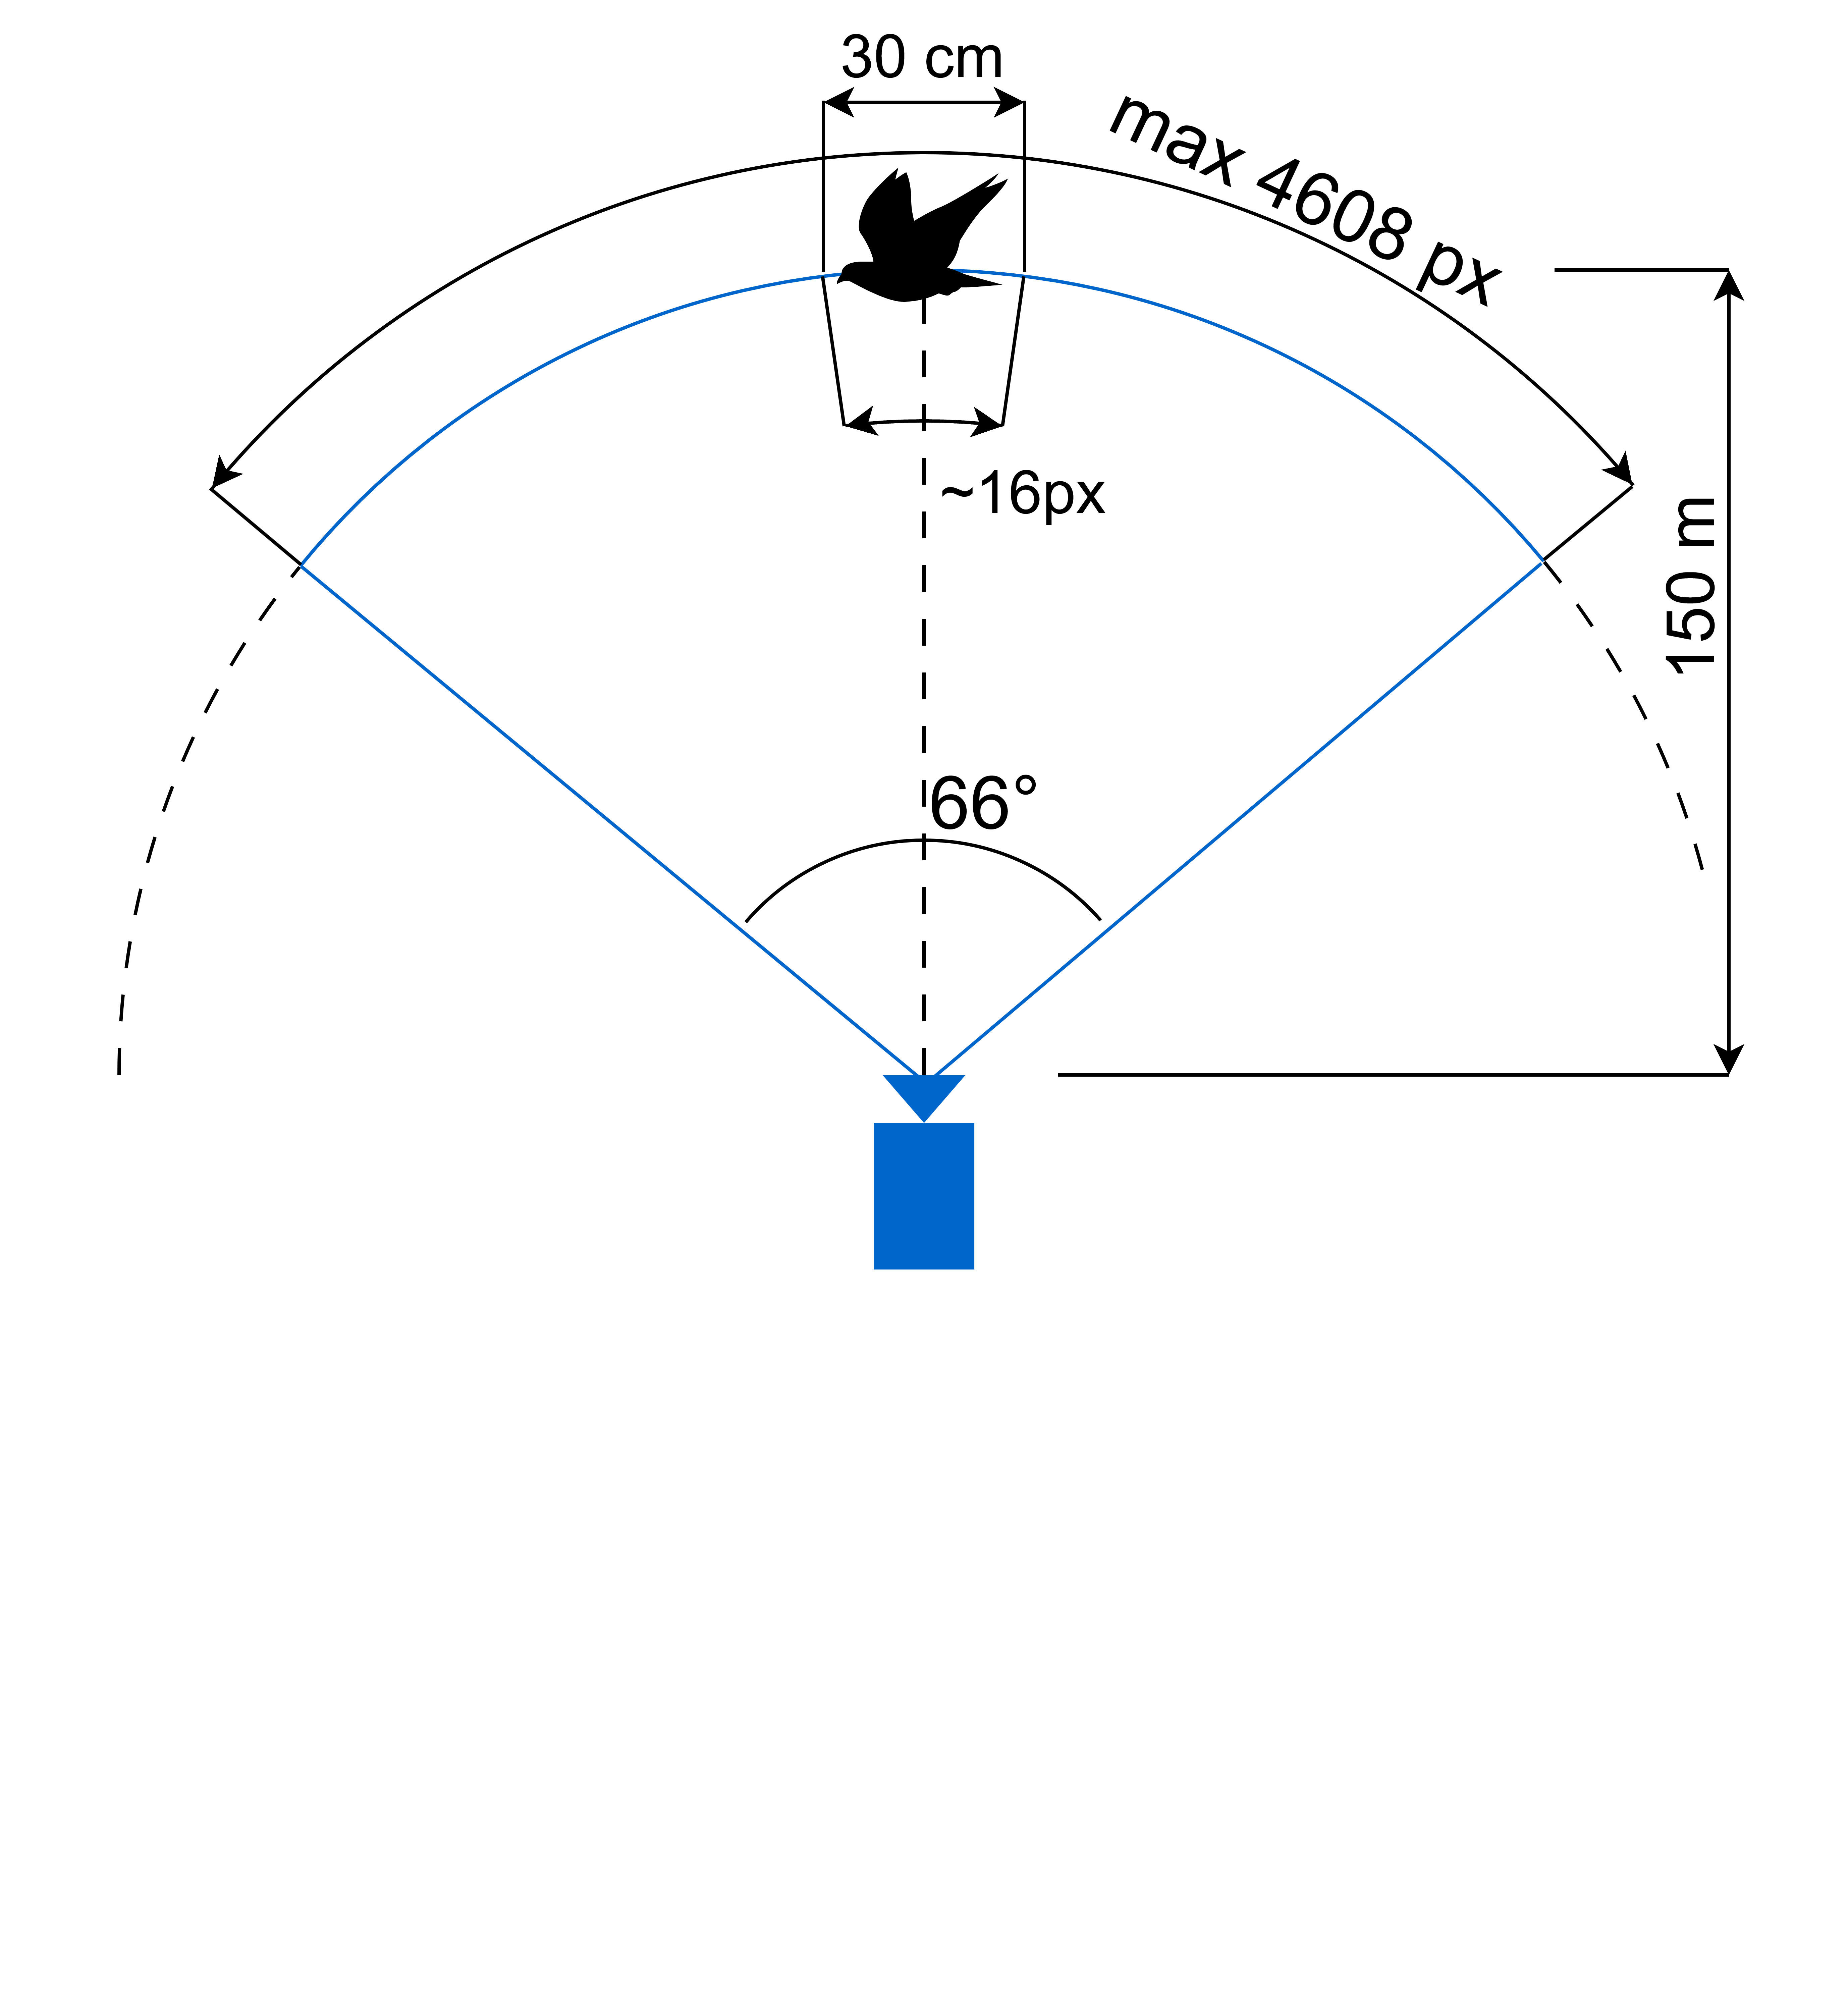
\includegraphics[width=.6\textwidth]{obrazky/camera/fov.drawio.png}
            \caption{Rozlíšenie kamery}
        \end{figure}

    \section{Ovládacie prvky}

        Ako najlepší ovládací a zobrazovací prvok bol z hľadiska prenosnosti a kompaktnosti zvolený dotykový displej, konkrétne 7 palcový IPS displej od firmy Waveshare. Táto veľkosť je postačujúca na zobrazovanie výsledkov detekcie aj ovládanie zariadenia. Rozhranie HDMI značne zjednodušuje prepojenie a inštaláciu displeja.

    \section{Uchytenie kamery}

        Praktickou výhodou prenosného zariadenia je možnosť jeho umiestnenia na statív. Keďže cieľom je kamerou mieriť smerom nahor na oblohu, bolo by užívateľské rozhranie pri nesprávne navrhnutej orientácii kamery a displeja natočené neprakticky nadol. Namiesto pevnej konfigurácie uhla medzi displejom a kamerou bolo navrhnuté pohyblivé uchytenie kamery v kryte zariadenia vyrobiteľné 3D tlačou.

        \begin{figure}[H]
            \centering
            \begin{tikzpicture} [node distance=7cm, auto]
                \node (image1) {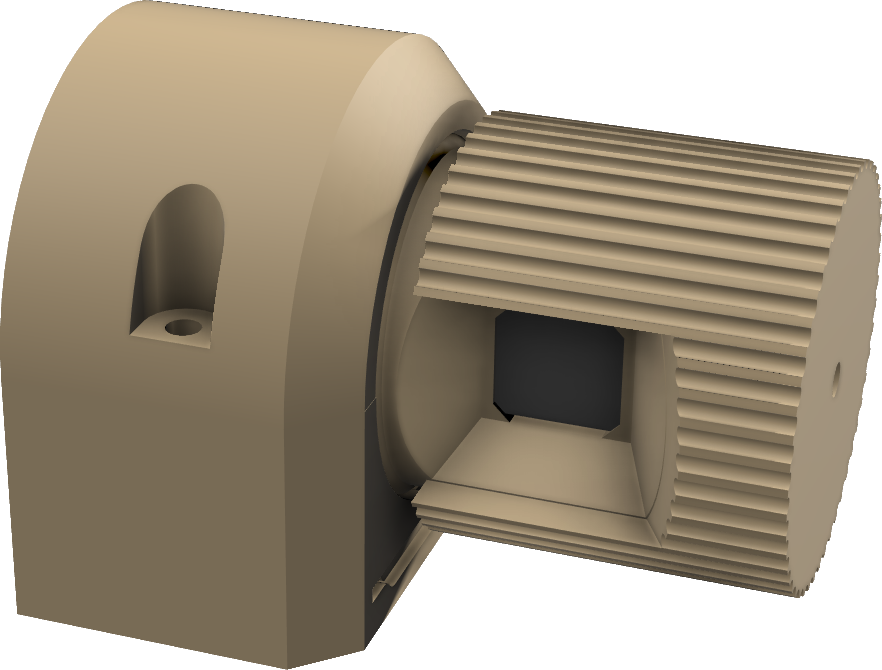
\includegraphics[width=.18\textwidth]{obrazky/case/camera_1.png}};
                \node (image2) [right of=image1] {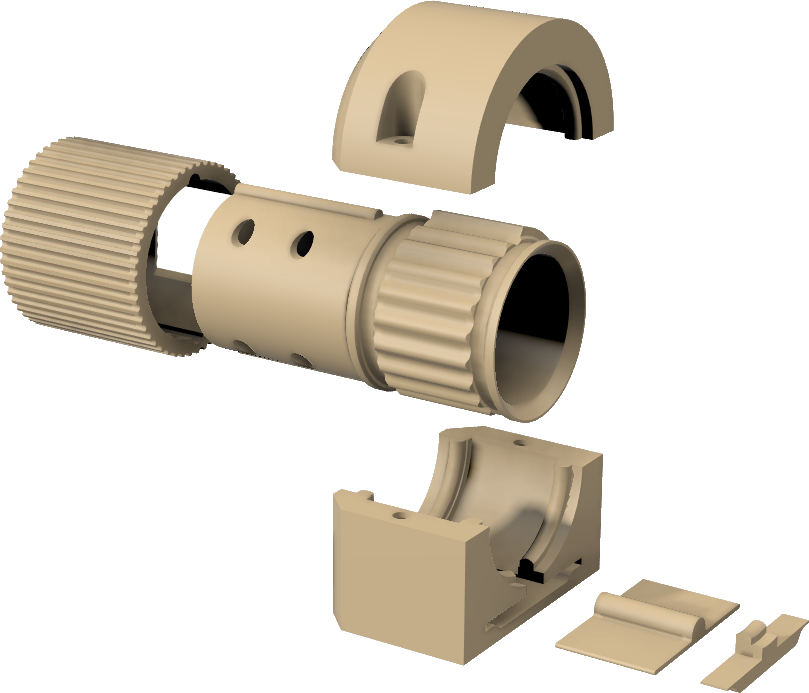
\includegraphics[width=.45\textwidth]{obrazky/case/camera_2.png}};
            \end{tikzpicture}
            \caption{Návrh nastaviteľného uchytenia kamery}
        \end{figure}

        \begin{figure}[h]
            \centering
            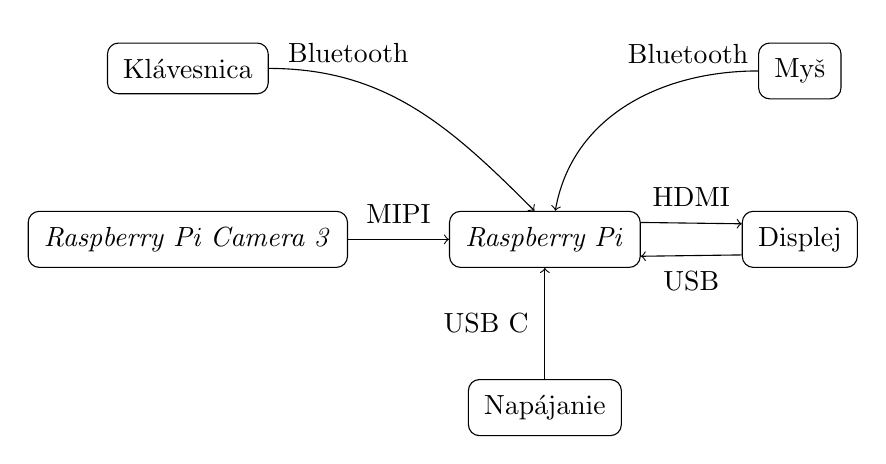
\begin{tikzpicture} [node distance=2.5cm, auto, inner sep=.2cm, rounded corners]
                \node (Pi) [draw, rectangle] at(0,0) {\emph{Raspberry Pi}};
                \node (Display) [right of=Pi, draw, rectangle, anchor=west] {Displej};
                \node (Camera) [left of=Pi, draw, rectangle, anchor=east] {\emph{Raspberry Pi Camera 3}};
                \node (Power) [below of=Pi, draw, rectangle, anchor=south] {Napájanie};
                \node (Keyboard) [above of=Camera, draw, rectangle, anchor=north] {Klávesnica};
                \node (Mouse) [above of=Display, draw, rectangle, anchor=north] {Myš};

                \draw[->] (Pi.10) -- (Display.165) node[midway, above] {HDMI};
                \draw[->] (Display.195) -- (Pi.350) node[midway, below] {USB};
                \draw[->] (Camera) -- (Pi) node[midway, above] {MIPI};
                \draw[->] (Power) -- (Pi) node[midway, left] {USB C};
                \draw[->] (Keyboard.east) to [out=. in=100] node[near start, above]{Bluetooth} (Pi.110);
                \draw[->] (Mouse.west) to [out=180, in=80] node[near start, above]{Bluetooth} (Pi.70);
            \end{tikzpicture}
            \caption{Bloková schéma zariadenia}
        \end{figure}

    \section{Kryt zariadenia}
        Kryt zariadenia sa skladá z troch hlavných častí. Jednotlivé komponenty zariadenia sú upevnené ku spoločnej stredovej doske. Tá má zaistiť pevné spojenie komponentov. Z prednej strany dosky je pripevnený displej. Ten je prepojený ku \emph{Raspberry~Pi} na druhej strane stredovej dosky, na ktorej je na jednej strane vytvorený výrez na HDMI a USB káble. Na druhej strane je zároveň umiestnená batéria napájajúca \emph{Raspberry Pi}. Displej je napájaný cez USB pripojené k \emph{Raspberry Pi}, pomocou ktorého zároveň komunikuje jeho dotyková plocha.

        \begin{figure}[H]
            \centering
            \begin{tikzpicture} [node distance=7cm, auto]
                \node (image1) {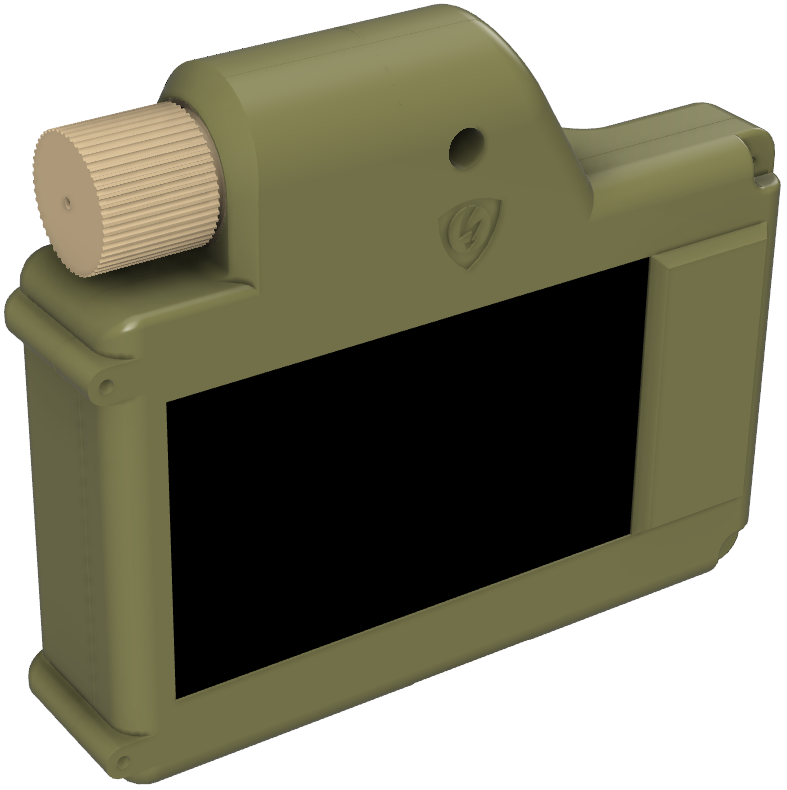
\includegraphics[width=.45\textwidth]{obrazky/case/pi camera device front view.png}};
                \node (image2) [right of=image1] {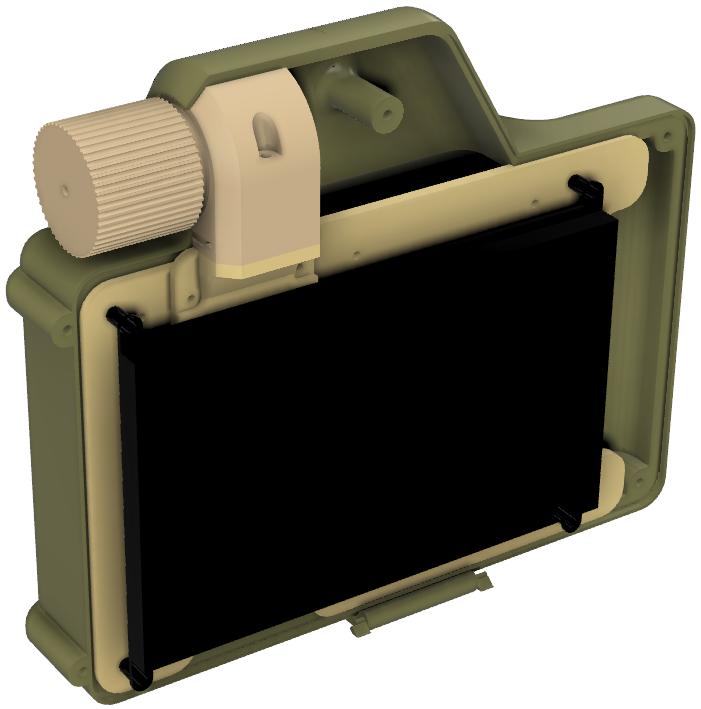
\includegraphics[width=.45\textwidth]{obrazky/case/pi camera device transparent front.png}};
            \end{tikzpicture}
            \caption{Pohľad na zariadenie spredu}
        \end{figure}

        \begin{figure}[H]
            \centering
            \begin{tikzpicture} [node distance=7cm, auto]
                \node (image1) {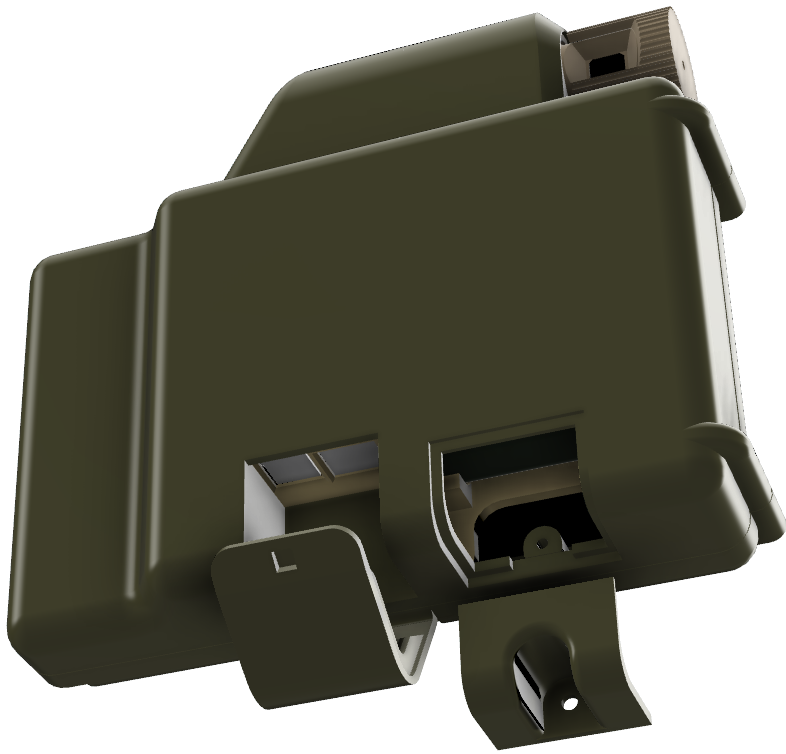
\includegraphics[width=.45\textwidth]{obrazky/case/pi camera device back cover opened.png}};
                \node (image2) [right of=image1] {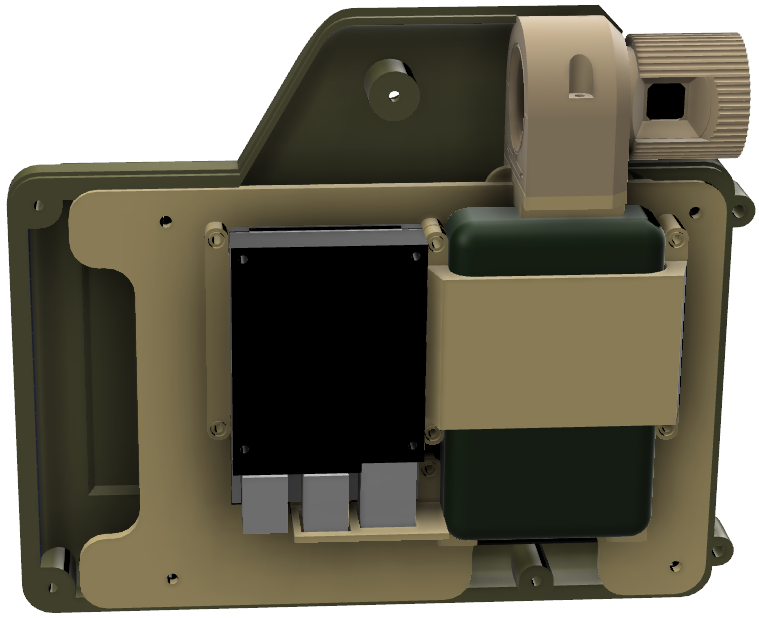
\includegraphics[width=.45\textwidth]{obrazky/case/pi camera device back transparent.png}};
            \end{tikzpicture}
            \caption{Pohľad na zariadenie zo zadu, s odnímateľnými krytmi}
        \end{figure}

        Hlavná doska je vložená medzi prednú a zadnú časť vonkajšieho krytu. Vonkajší kryt obklopuje celé zariadenie, okrem vnútorne nevyužitých USB výstupov \emph{Raspberry Pi} a batérie. Tie sú prístupné za odnímateľnými krytmi.  

\chapter{Tvorba datasetu}

    Správne naučenie modelov a ich schopnosť generalizovať z veľkej miery záleží na~kvalite použitého datasetu (množiny dát). Tvorba datasetu je teda kľúčový krok pri~práci so systémami strojového videnia.

    Cieľom pri tvorbe datasetu je zabezpečiť dostatočnú kvalitu a správnosť dát, dosiahnuť početne podobné zastúpenie každej triedy a správne reprezentovať rôznorodosť dát v rámci jednotlivých tried. Je vhodné, aby boli vzorky získané pri rôznych podmienkach podľa plánovaného použitia výsledného modelu.

    \section{Získavanie dát}

        Keďže táto práca nadväzuje na~prácu \cite{Jurecka2021}, tvorí dataset v~nej vytvorený základ pre~dataset použitý v~tejto práci. Navyše bol rozšírený o~niekoľko ďalších open source datasetov a~vlastných anotovaných fotografií.

        Na~tvorbu datasetu bol použitý program \emph{roboflow}, ktorý umožňuje načítavanie existujúcich datasetov, nahrávanie vlastných fotografií, anotáciu, spájanie dostupných datasetov, augmentáciu datasetu a~generovanie anotačných súborov rôznych formátov.

        Práca s~programom \emph{roboflow} postupuje v~krokoch:

        \begin{enumerate}
            \item Vytvorenie projektu. Projekt programu \emph{roboflow} zahŕňa snímky, ich anotáciu a~vygenerovaný výstup spolu s~augmentáciou.

            \begin{figure}[H]
                \centering
                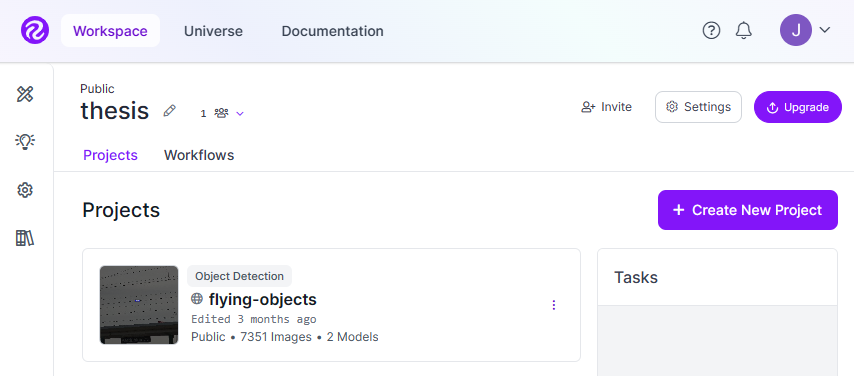
\includegraphics[width=.5\textwidth]{obrazky/roboflow/projects.png}
                \caption{Založenie roboflow projektu}
            \end{figure}

            \item Definícia tried anotovaných objektov. V~prípade vloženia cudzích datasetov je možné spojiť triedy s~rôznym názvom, ktoré majú reprezentovať rovnakú triedu objektu. Triedam sú priradené farby pre~ľahšie rozlíšenie objektov pri~ručnej anotácii.

            \begin{figure}[H]
                \centering
                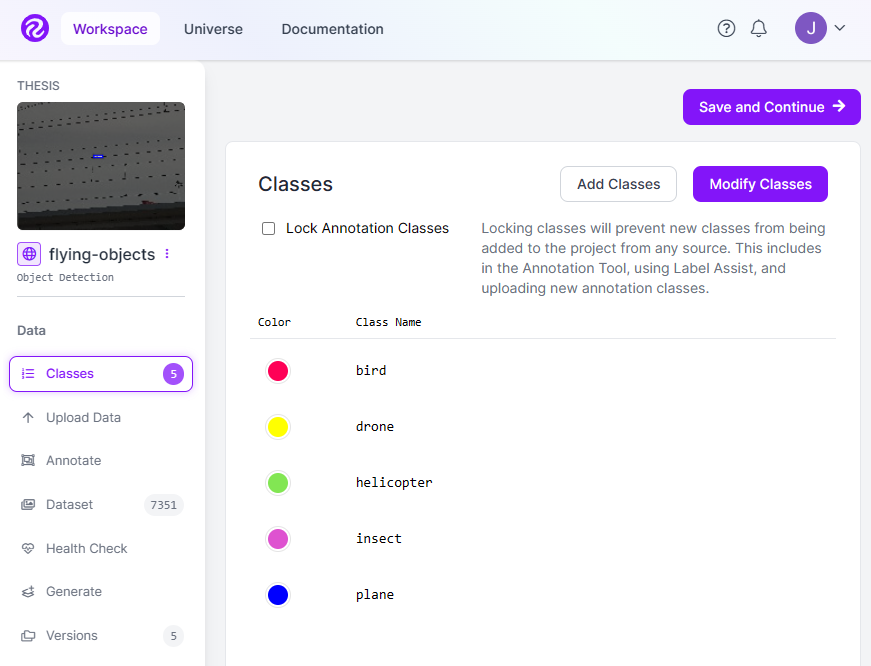
\includegraphics[width=.5\textwidth]{obrazky/roboflow/classes edit.png}
                \caption{Definícia tried roboflow projektu}
            \end{figure}

            \item Nahratie vlastných fotografií alebo naklonovanie existujúceho datasetu. Takto importovať je možné snímky spolu aj~s~anotáciou v~prípade, že~je už~vytvorená v~kompatibilnom formáte.

            \item Ručná anotácia. Pre použitie v~tejto práci bola vytvorená anotácia obdĺžnikovým orámovaním objektov so~zaradením do~tried.

            \begin{figure}[H]
                \centering
                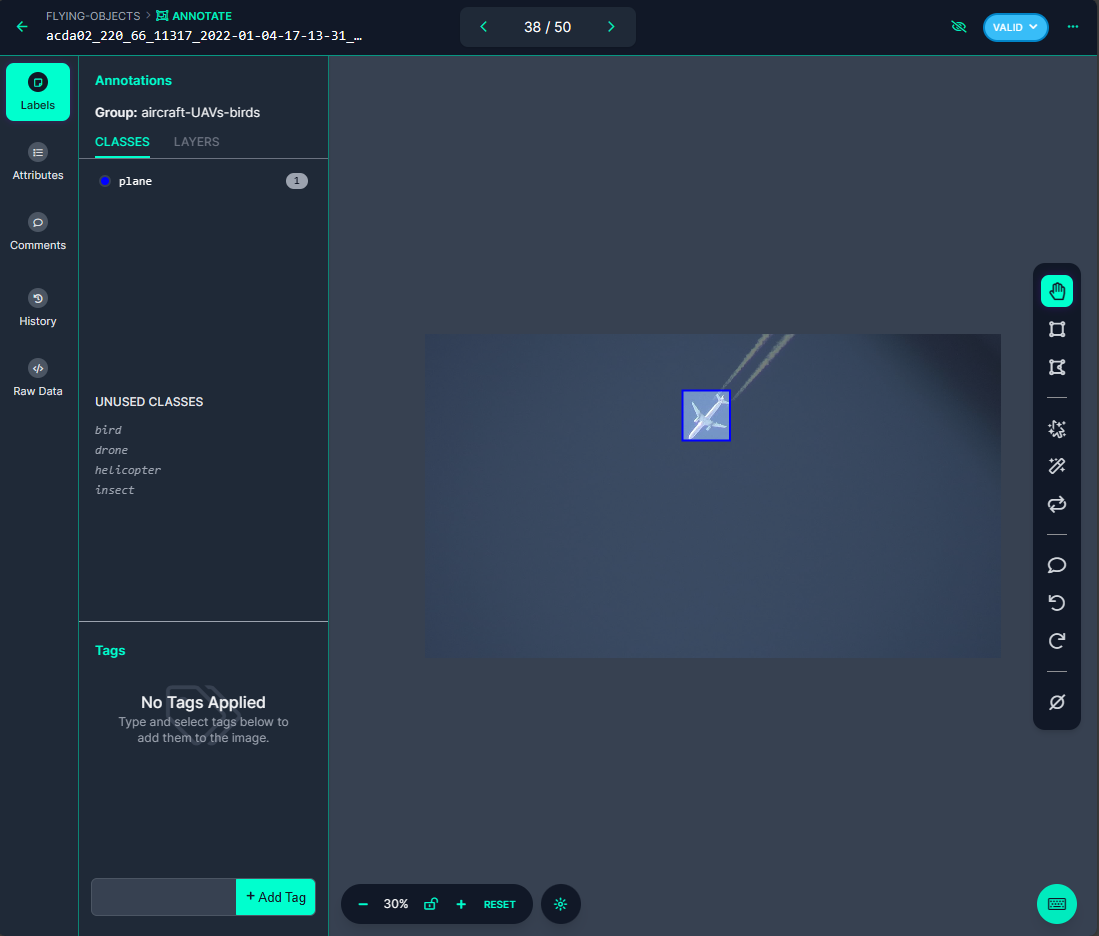
\includegraphics[width=.5\textwidth]{obrazky/roboflow/annotate.png}
                \caption{Anotácia snímku v programe roboflow}
            \end{figure}

            \item Kontrola, nastavenie a~vygenerovanie novej inštancie datasetu. Pred stiahnutím archívu s~anotovaným datasetom je potrebné nastaviť parametre ako~je požadované rozlíšenie a spôsob zarovnania tvaru snímok (čierne pozadie, výrez, roztiahnuť, zrkadlenie). Taktiež je možné aplikovať nastavené randomizované augmentácie na~náhodne vybrané snímky z~trénovacieho datasetu. Po nastavení počtu generovaných snímok je možné vygenerovať a stiahnuť dataset.

            \begin{figure}[H]
                \centering
                \includegraphics[width=.5\textwidth]{obrazky/roboflow/dataset generate.png}
                \caption{Generované verzie datasetu v roboflow}
            \end{figure}

        \end{enumerate}

        Po pridaní všetkých častí datasetu a~kontrole správnosti anotácie boli počty inštancií jednotlivých tried v trénovacom datasete:

        \begin{itemize}
            \item \textbf{vták}: 1198
            \item \textbf{dron}: 1898
            \item \textbf{helikoptéra}: 1281
            \item \textbf{hmyz}: 934
            \item \textbf{lietadlo}: 972
        \end{itemize}

        \begin{figure}[H]
            \centering
            \begin{tikzpicture} [node distance=.001\textwidth]
                \node (image1) {\includegraphics[width=.23\textwidth]{obrazky/roboflow/image_examples/h1.png}};
                \node (image2) [right=of image1] {\includegraphics[width=.23\textwidth]{obrazky/roboflow/image_examples/h2.png}};
                \node (image3) [right=of image2] {\includegraphics[width=.23\textwidth]{obrazky/roboflow/image_examples/p1.png}};
                \node (image4) [right=of image3] {\includegraphics[width=.23\textwidth]{obrazky/roboflow/image_examples/p2.png}};
                \node (image5) [below=of image1] {\includegraphics[width=.23\textwidth]{obrazky/roboflow/image_examples/b1.png}};
                \node (image6) [below=of image2] {\includegraphics[width=.23\textwidth]{obrazky/roboflow/image_examples/b2.png}};
                \node (image7) [below=of image3] {\includegraphics[width=.23\textwidth]{obrazky/roboflow/image_examples/i1.png}};
                \node (image8) [below=of image4] {\includegraphics[width=.23\textwidth]{obrazky/roboflow/image_examples/i2.png}};
                \node (image9) [below=of image6] {\includegraphics[width=.23\textwidth]{obrazky/roboflow/image_examples/d1.png}};
                \node (image10) [below=of image7] {\includegraphics[width=.23\textwidth]{obrazky/roboflow/image_examples/d2.png}};
            \end{tikzpicture}
            \caption{Ukážka niekoľkých snímok z datasetu}
        \end{figure}


    \section{Úprava, rozdelenie a rozšírenie datasetu}

        Niektoré triedy sú reprezentované výrazne menším množstvom jednotlivých inštancii, čo je spôsobené nižšou dostupnosťou dát. Väčšina fotografii vtákov zo vzdialenosti, pri ktorej by mali byť detekované, pochopiteľne obsahuje niekoľko desiatok jedincov, trieda vták je teda nadmerne zastúpená. Je možné tento problém čiastočne vyriešiť augmentáciou datasetu, čo program \emph{roboflow} umožňuje priamo pri generovaní novej verzie. V budúcnosti je vhodnejším riešením ďalšie rozšírenie datasetu o snímky s~objektami aktuálne nedostatočne reprezentovaných tried.

        Aby bolo zabránené preučeniu modelu, musia byť dáta, na ktorých je model učený, rôzne od validačných a testovacích. Anotované obrazové dáta boli rozdelené do skupín s počtom:

        \begin{itemize}
            \item \textbf{trénovanie}: 2367
            \item \textbf{validácia}: 572
            \item \textbf{testovanie}: 290
        \end{itemize}

        Snímky boli predspracované upravením veľkosti na \(640 \times 640\) px a boli aplikované augmentácie, ktorými bol počet inštancií v trénovacej množine rozšírený na 7101:

        \begin{itemize}
            \item Rotácia \(-30^\circ\) až \(+30^\circ\)
            \item Zkosenie \(\pm 15^\circ\) vertikálne aj horizontálne
            \item Posun odtieňu \(-35^\circ\) až \(+35^\circ\)
            \item Zmena saturácie -25 \% až +25 \%
            \item Zmena expozície -20 \% až +20 \%
            \item Rozmazanie do 0,8 px
        \end{itemize}

    \section{Testovanie použiteľnosti datasetu}

    Použiteľnosť modelu bola testovaná naučením modelu typu \emph{Roboflow 3.0 Object Detection} priamo v aplikácii \emph{roboflow}, ktorý dosahoval úroveň presnosti 86.1 \% pri~zvolenom variante modelu \emph{fast}. Pri dlhšom učení modelu určeného na reálne použitie sa dá predpokladať, že dosiahnutá presnosť bude vyššia.

    Obrázok \ref{fig:roboflow_metrics} zobrazuje metriky presnosti naučeného modelu vypočítané v programe \emph{roboflow} tak, ako sa v ňom zobrazujú. Vypočítané metriky sú:

    \begin{itemize}
        \item \textbf{\ac{mAP}} \\ priemer priemerných presností za všetky triedy.
        \item \textbf{Presnosť (Precision)}.
        \item \textbf{Senzitivita (Recall)}.
    \end{itemize}

    \begin{figure}[H]
        \centering
        \includegraphics[width=.35\textwidth]{obrazky/roboflow/metrics.png}
        \caption{Metriky presnosti naučeného modelu v programe roboflow}
        \label{fig:roboflow_metrics}
    \end{figure}

    \begin{figure}[H]
        \centering
        \includegraphics[width=.8\textwidth]{obrazky/roboflow/train.png}
        \caption{Grafické zobrazenie priebehu učenia modelu roboflow}
    \end{figure}

    Výsledná vygenerovaná verzia datasetu je z programu exportovateľná v niekoľkých formátoch, napríklad pre učenie siete \ac{YOLO} alebo pre použitie s knižnicou \emph{tensorflow}. Pri exporte je stiahnutý komprimovaný priečinok obsahujúci obrazové dáta a anotáciu.

    \begin{figure}[H]
        \centering
        \includegraphics[width=.5\textwidth]{obrazky/roboflow/export.png}
        \caption{Exportovanie vytvoreného datasetu}
    \end{figure}

\chapter{Návrh softvéru}

    Pri návrhu a tvorbe aplikácie systému detekcie lietajúcich objektov bol kladený dôraz na:
    \begin{itemize}
        \item spustiteľnosť a použiteľnosť na počítači,
        \item ovládateľnosť dotykovým panelom,
        \item modulárnosť a rozšíriteľnosť,
        \item spätná väzba a grafické zobrazenie výsledkov užívateľovi,
        \item možnosť používať, testovať a porovnávať rôzne metódy detekcie, klasifikácie a~trasovania.
    \end{itemize}

    \section{Použitý jazyk a knižnice}

        Použitím programovacieho jazyka \emph{python} bola získaná kompatibilita zo zariadeniami a operačnými systémami, ktoré podporujú interpretér jazyka \emph{python}, teda hlavne \emph{Raspberry Pi} s nainštalovaným operačným systémom Raspberry Pi OS a~osobné počítače, čo uľahčuje vývoj aplikácie a umožňuje jeho použitie na ľubovoľnom počítači.

        Na tvorbu grafického rozhrania bola použitá knižnica \ac{tkinter}. Tá umožňuje vytvárať grafické používateľské rozhranie priamo z kódu v jazyku \emph{python}. Obsahuje tiež objekty časovačov, vďaka ktorým je~možné jednoducho a spoľahlivo ovládať kontinuálny beh aplikácie. Užívateľské rozhranie vytvorené knižnicou \ac{tkinter} je kompatibilné s ovládaním klávesnicou a myšou, aj dotykovým displejom.

        Knižnica \emph{OpenCV} obsahuje implementáciu množstva algoritmov spracovania obrazu a počítačového videnia. Umožňuje základné operácie s videom aj jednotlivými snímkami ako načítanie, ukladanie a zobrazovanie, pričom podporuje rôzne formáty obrazových dát. Sofistikovanejšie úlohy, ktoré knižnica rieši, zahrňujú detekciu, klasifikáciu, sledovanie pohybu. Knižnica \emph{OpenCV} je kompatibilná s viacerými programovacími jazykmi, vrátane jazyku \emph{python}.

    \section{Štruktúra aplikácie}
        Aplikácia systému je zložená z~automaticky načítavaných modulov. Každý z~modulov predstavuje časť reťazca spracovania obrazu a~detekcie objektov v~ňom. Program patriaci každému modulu je vykonávaný v~samostatnom vlákne, vďaka čomu nemusia moduly čakať na~vykonanie nasledujúceho modulu a~namiesto toho môžu spracovávať ďalší snímok v~poradí.

        Jedným z~modulov, ktoré sú vždy aktívne, je modul reprezentujúci zoznam aktívnych modulov. Ten je zodpovedný za~načítavanie a~spúšťanie modulov, distribúciu dát medzi modulmi a~ukladanie a~načítavanie konfigurácie modulov.
        \subsection{Štruktúra modulu aplikácie}
            Každý z automaticky načítavaných modulov dedí od abstraktnej triedy \\ modules.ModuleBase. Tá predpisuje spoločnú časť správania modulov, menovite:

            \begin{itemize}
                \item \textbf{Prvky užívateľského rozhrania týkajúce sa modulu:}
                \begin{itemize}
                    \item záznam v zozname typov modulov,
                    \item užívateľské rozhranie s nastaveniami modulu,
                    \item záznam v zozname aktívnych inštancií modulov.
                \end{itemize}
                \item \textbf{Zoznam konfiguračných metód.} Tie sú využívané pri získavaní konfigurácie z~modulu a~jej vloženie do~modulu pri~jeho spustení. Priamo v~kóde modulu sú konfiguračné metódy definované ako~bežné metódy, ktoré prijímajú ako~voliteľný vstup novú hodnotu v~prípade, že je požadovaná zmena a~vracajú aktuálnu hodnotu určitého nastavenia modulu. Automatické spúšťanie ukladania konfigurácie pri zmene nastavenia a~opätovné načítavanie konfigurácie je dosiahnuté implementáciou dekorátora, ktorým sú konfiguračné metódy označené. Pri definícii triedy sú automaticky vložené jej označené konfiguračné metódy do~zoznamu spoločného pre všetky moduly, kde sú priradené danému modulu. Pri volaní konfiguračnej metódy sa spúšťa wrapper metóda definovaná v dekorátore, úlohou ktorej je zmena uloženej hodnoty v~konfiguračnom súbore.
                \item \textbf{Unikátnu identifikáciu modulu} pridelenú automaticky pri vytvorení novej inštancie modulu.
                \item \textbf{Určenie typu vstupných aj výstupných dát.} To umožňuje niektorým modulom vedieť, aké dáta môžu očakávať a~užívateľskému rozhraniu aké dáta je možné vizualizovať.
                \item \textbf{Vstupnú frontu}, do~ktorej sú vkladané objekty obsahujúce kolekciu dát priradených k~jednotlivým typom dát, ktoré modul definuje ako svoje vstupy a~výstupy. Objekt s~dátami je pri jeho vzniku vložený ako referencia do~fronty každého z~modulov, ktoré potom čakajú na~dostupnosť ich požadovaných dát. Po získaní vstupu je vykonaná činnosť modulu a~do~objektu z~fronty  sú pridané výstupné dáta. Keďže sú objekty do~vstupných front predávané referenciou, dáta sú po~ich pridaní dostupné aj v~ostatných moduloch. Aby bolo čakanie efektívne, je pri~pridaní dát nastavený \emph{threading.Event}, ktorý zobudí čakajúce moduly. Modul má dostupné funkcie na~nahliadnutie do~fronty, získanie nasledujúceho objektu z~fronty a~vloženie nového objektu do~front všetkých aktívnych modulov, ktoré očakávajú vstup.
                \item \textbf{Konzolový výstup.} Každému modulu je predaný objekt reprezentujúci konzolový výstup. Výpis do konzoly je vždy uvedený spolu s~názvom a~ID modulu, a~časovou značkou. Konzolový výstup je vykonávaný v~samostatnom vlákne, moduly teda nečakajú na~dokončenie výpisu a~súčasný výpis z~viacerých modulov nespôsobí nesprávny formát výstupu. Výstup podporuje konzolové farby pomocou escape sekvencií a~farebne rozlišuje informatívny, varovný, chybový výstup, a~výstup informujúci o~nastavení modulov. Názov modulu a časová značka je tiež farebne rozlíšená.
                \begin{figure}[H]
                    \centering
                    \begin{lstlisting}
module list : 46abbe6c - 16:08:17 - creating module
module list : 46abbe6c - 16:08:17 - finished creating
module list : 46abbe6c - 16:08:17 - looking for modules
in background_model.py
module list : 46abbe6c - 16:08:17 - importing module
object BackgroundModel
                    \end{lstlisting}
                    \caption{Príklad výstupu pri spustení aplikácie}
                \end{figure}
                \item \textbf{Inicializačné vlákno} spustené pri inicializácii modulov, ktoré je zodpovedné za~prvotné nastavenie modulu.
                \item \textbf{Aktívne vlákno} je spustené pri aktivácii modulov, ktoré v~slučke získava, spracováva vstupné dáta a~ukladá výstupné dáta. Toto vlákno počas života objektu neskončí, ak~nedôjde k~nezachytenej výnimke.
                \item \textbf{Timeout dát.} Každému objektu vo vstupnej fronte je priradený čas jeho vzniku. Keď sa ich modul pokúša z fronty čítať, sú preskočené všetky objekty staršie ako určený čas.
            \end{itemize}

            Aplikácia automaticky načíta všetky moduly definované v~súboroch uložených v~priečinku \emph{autoload\_modules} použitím python knižnice importlib. Výberom modulu zo~zoznamu dostupných modulov je vytvorená nová inštancia modulu. Na nej je možné zmeniť konfiguráciu pred~vložením inštancie do~zoznamu aktívnych modulov.

        \subsection{Implementované moduly}
            Do aplikácie boli implementované nasledujúce moduly:
            \begin{itemize}
                \item \textbf{Zdroj obrazu:} Tento typ modulu získava nové obrazové dáta. Následne môže vytvárať šedotónový obraz, pričom je možné určiť váhy farebných zložiek. Nakoniec je možne vykonávať prahovanie, a~to buď s~nastaveným alebo s~automaticky určeným prahom. Existujú dva varianty: 
                \begin{itemize}
                    \item \textbf{Video:} V~nastaveniach modulu videa ako zdroja obrazu je možné okrem spoločných nastavení pre~všetky zdroje určiť aj cestu k~súboru videa. Po pridaní do~zoznamu aktívnych modulov a~spustení, tento modul začne pridávať obrazové dáta do~fronty so~snímkovacou frekvenciou, akú má zdrojové video.
                    \item \textbf{Kamera:} Ak~je v~prostredí, v~ktorom aplikácia beží dostupná python knižnica PyCamera2, ktorá slúži na~ovládanie kamery a~získavanie snímok z~nej, je možné pridať modul kamery. Ten má možnosť nastaviť rozlíšenie kamery.
                \end{itemize}
                \item \textbf{Dynamický model pozadia:} Generuje postupne sa~aktualizujúci model pozadia, s~ktorým potom vypočíta absolútnu hodnotu rozdielu s~aktuálnou snímkou. Ten je potom prahovaný nastavenou hodnotou, čím vzniká binárny obraz, v~ktorom je možné detegovať pohybujúce sa~objekty. Nastaviť je v~tomto module možný prah, ktorý keď prekročí úroveň pohybu v~obraze, prestane sa~aktualizovať model pozadia. Nastaviteľné prahy sú dva, prah dvoch po~sebe nasledujúcich snímkov a~prah medzi snímkou a~modelom pozadia. Ich úroveň je určená relatívne k~rozlíšeniu obrazu a~normalizovaná na~maximálnu úroveň jasu jedného pixelu, čím je získaná nezávislosť na~rozlíšení a~číselnej reprezentácii obrazu. Ďalšie nastavenia zahŕňajú časovú konštantu zmeny pozadia, spolu s~maximálnou zmenou jasu každého pixelu za~jednu iteráciu. 
                \item \textbf{Generátor orámovaní z binárneho obrazu:} Vyhľadáva súvislé oblasti v~binárnom obraze a~vytvára obdĺžnikové orámovania. Pred vyhľadávaním najprv vykoná morfologické zatvorenie s~cieľom spojiť blízke oblasti, ktoré pravdepodobne patria jednému objektu. Tvar jadra zatvorenia je možné nastaviť. Oblasti s menším počtom pixelov ako nastavený prah sú ignorované.
                \item \textbf{Tensorflow klasifikácia:} Načíta uložený naučený klasifikačný model vo~formáte keras. Vďaka tomu je možné použiť na výpočty GPU na zariadeniach, kde je dostupná, nainštalovaním GPU verzie knižnice tensorflow. Tomuto modulu je potrebné nastaviť cestu k~súboru s~uloženým modelom. Načítaný model je potom aplikovaný na~vystrihnuté oblasti podľa orámovaní z~pôvodného farebného obrazu. Očakávaný je výstup typu one-hot, teda každý výstup určuje predpokladanú pravdepodobnosť zaradenia objektu v~orámovaní do~triedy asociovanej s~daným výstupom. Výsledná klasifikácia je zvolená ako~trieda s~najvyššou pravdepodobnosťou, ak~presahuje určený prah. Modely pre~tento modul boli vytvorené v~prostredí matlab deep network designer, naučené pomocou transfer learning a~exportované do~formátu pre tensorflow keras. Boli použité predučené konvolučné siete Resnet50, Squeezenet a~Googlenet.
                \item \textbf{YOLO detektor:} Reprezentuje detekčnú sieť YOLOv8 schopnú detekcie objektov aj~ich klasifikácie v~jedinom kroku. Pri~použití tohto modulu teda nie~je nutné pridávať iné moduly detekcie. Výstup modelov YOLO je taktiež one-hot, výsledná klasifikácia funguje teda rovnako ako vo~vyššie popísanom module tensorflow klasifikátorov. Spolu s~klasifikáciou vracia tento modul aj~samotné orámovanie detegovaných objektov.
                \item \textbf{Záznam videa:} Získané snímky je možné týmto modulom ukladať do súboru videa. Spolu s~videom sú ukladané orámovania detegovaných potenciálnych objektov. Ak~je dostupný modul generujúci orámovania, sú ukladané len snímky s~potenciálnym výskytom objektu.
            \end{itemize}

    \section{Automatické spúšťanie aplikácie}
        Zjednodušením používania zariadenia je zaistenie automatického spustenia aplikácie systému detekcie pri~zapnutí zariadenia. Toho bolo dosiahnuté nastavením aplikácie ako~servisu operačného systému \emph{Raspberry~Pi~OS}, ktorý je nainštalovaný na~\emph{Raspberry~Pi} na~zariadení.

        Servisy sú v~systéme \emph{Raspberry~Pi~OS} spravované servisovým manažérom \emph{Systemd}. Definované sú v~konfiguračných súboroch, takzvaných \emph{systemd unit files}, uložených v~priečinku \path{/etc/systemd/system/}. Konfigurácia je v týchto súboroch rozdelená do sekcií. Najdôležitejšiou sekciou je sekcia [Service], obsahujúca informácie o spustení aplikácie. Tu je nutné definovať pracovný priečinok aplikácie, príkaz spustenia a spôsob reštartovania v prípade nečakaného ukončenia aplikácie. Aby mala aplikácia prístup ku~potrebným knižniciam, je nutné použiť virtuálne prostredie \emph{python} s nainštalovanými knižnicami. V konfigurácii spustenia aplikácie je nutné použiť \emph{python} interpretér nainštalovaný v tomto virtuálnom prostredí.

        \begin{figure}[H]
            \centering
            \begin{lstlisting}
[Service]
Type=simple
WorkingDirectory=<cesta ku pracovnému priečinku>
ExecStart=<python interpreter> <skript aplikácie>
Restart=always
User=<užívateľ>
            \end{lstlisting}
            \caption{Sekcia [Service] konfigurácie automatického spustenia aplikácie}
        \end{figure}

    \section{Návrh grafického rozhrania}
        \ac{GUI} umožňuje intuitívne ovládanie aplikácie~a zobrazovanie výsledkov detekcie a~klasifikácie. Ovládanie aplikácie je rozdelené do~záložiek. V~ľavej časti obrazovky je zobrazený aktuálny snímok s~výstupom detekcie a~klasifikácie. Zobrazujú sa v~ňom orámovania detegovaných objektov a~ich priradenie do~tried. Prvá záložka (\emph{Results}) zobrazuje aktuálny snímok spolu s~vybranou vizualizáciou.

        \begin{figure}[H]
            \centering
            \includegraphics[width=\textwidth]{obrazky/new_app/classification.png}
            \caption{Záložka na~zobrazenie výstupov detekcie}
        \end{figure}

        Zobraziteľné dáta zahrňujú:
        \begin{itemize}
            \item \textbf{Pôvodný farebný obraz} získaný z~videa alebo kamery.
            \item \textbf{Šedotónový obraz} vytvorený lineárnou kombináciou farebných zložiek pôvodného obrazu. Je využívaný pri detekcii prahovaním.
            \item \textbf{Aktuálny model pozadia} slúžiaci na~detekciu objektov pohybom.
            \item \textbf{Binárny obraz}, v~ktorom sú označené oblasti potenciálneho výskytu objektu.
            \item \textbf{Orámovanie oblastí} s~potenciálnym výskytom objektu. 
            \item \textbf{Klasifikácia oblasti} s~ farebným zvýraznením orámovaní a~zobrazením názvu tried.
        \end{itemize}

        Zoznam na~pravej strane obrazovky obsahuje prepínače rozhodujúce o~tom, ktoré z~možných  zobraziteľných dát sú vľavo vykresľované. V~zozname sú zobrazené len prepínače pre~tie typy dát, ktoré sú produkované aktuálnymi aktívnymi modulmi.

        O tom, ktoré moduly sú aktuálne aktívne, rozhoduje užívateľ v druhej záložke (\emph{Modules}). 

        \begin{figure}[H]
            \centering
            \includegraphics[width=\textwidth]{obrazky/new_app/modules_window_motion_detection.png}
            \caption{Záložka na~nastavenie modulov}
        \end{figure}

        Rozhranie tejto záložky je rozdelené do troch stĺpcov posúvateľných vertikálne, keďže množstvo obsahu každého nie~je obmedzené. Ovládacie prvky v~každom\linebreak z~týchto stĺpcov sú definované v~súboroch spolu s~automaticky načítavanými modulmi.

        Stĺpec na~pravej strane obsahuje zoznam dostupných typov modulov. Po~kliknutí na~typ modulu je buď vytvorená nová inštancia modulu zvoleného typu, alebo aktívna inštancia, ak~už~pre tento typ jedna existuje. Takto získaná inštancia je potom predaná strednému stĺpcu.

        Stredný stĺpec obsahuje konfiguračné ovládacie prvky modulu. Zobrazuje sa~vždy nastavenie zvolenej inštancie, pričom zmena nastavení spustí uloženie novej konfigurácie do~yaml súboru. Kliknutím na~tlačidlo \emph{Save and~add module} je modul s~nastavenou konfiguráciou vložený do~zoznamu aktívnych modulov, ak~ide o~novovytvorenú inštanciu.
        
        V~ľavom stĺpci sa~nachádza zobrazenie aktívnych inštancii modulov. Kliknutím na záznam reprezentujúci aktívnu inštanciu modulu otvorí nastavenia tejto inštancie v strednom stĺpci, rovnako ako pri kliknutí na typ už aktívneho modulu v pravom stĺpci. Záznamy v ľavom stĺpci môžu zobrazovať dodatočné informácie, ako napríklad modul dynamického modelu pozadia, ktorý zobrazuje úroveň detekovaného pohybu, čo uľahčuje nastavenie prahov detekcie pohybu.

\chapter{Kontrola a porovnanie prístupov}
    Aby bolo možné porovnať rôzne prístupy k~detekcii a~klasifikácii, je nutné zozbierať reálne zábery z~použitej kamery.  Tie sú následne po~ručnom anotovaní predané jednotlivým typom detektorov. Detekcie je potom možné porovnať s~anotáciou a~získať tak rôzne metriky presnosti.
    \section{Zber dát}
        Reálne snímky z~kamery boli zbierané použitím modulu aplikácie nazvaného \emph{video capture}, teda zber videa.  Tento modul má za~úlohu ukladať snímky získané z~kamery, aj keď funguje rovnako aj so~snímkami z~uloženého videa.  Výstup je ukladaný do~video súboru vo~formáte mp4. V prípade, že je medzi aktívnymi modulmi aj modul vytvárajúci orámovania, sú ukladané len tie snímky, ktoré obsahujú aspoň jeden detegovaný potenciálny objekt, teda aspoň jedno orámovanie. Jednotlivé orámovania sú ukladané do~yaml súboru spolu s~indexom snímky, ku~ktorému patria.

        Na zber dát bol použitý modul pre vytváranie dynamického modelu pozadia a modul detekcie objektov z binárneho obrazu, ktorý vzniká prahovaním rozdielového obrazu s modelom pozadia. Detegované objekty sú orámované a predané modulu na zber videa.

    \section{Úprava dát}
        Pred použitím zozbieraných snímkov na~vyhodnotenie a~porovnanie prístupov k~detekcii je nutné ich najprv anotovať, prípadne upraviť nesprávne orámované objekty, či~falošne označené oblasti, ktoré objekt neobsahujú. Na~tento účel bola vytvorená aplikácia na~úpravu zbieraných videí.

        Táto aplikácia, na rozdiel od hlavnej aplikácie detekcie a klasifikácie, bola napísaná v jazyku \emph{C\char"0023}. Bol v nej použitý framework \emph{WPF (Windows Presentation Foundation)} pre \ac{GUI} a knižnica \emph{OpenCV}, ktorá bola použitá aj v hlavnej aplikácii.

        \begin{figure}[H]
            \centering
            \includegraphics[width=\textwidth]{obrazky/video_annotator/annotation_overview.png}
            \caption{Užívateľské rozhranie programu na anotáciu videa}
        \end{figure}

        Úprava videa začína načítaním súboru videa a~súboru so~zoznamom orámovaní. Užívateľ potom definuje triedy objektov nachádzajúcich sa v~otvorenom videu. Novú definíciu triedy do~zoznamu je možné pridať kliknutím na~zelené zvýraznené tlačidlo. Triede je potom možné priradiť poradové číslo a~názov. Červené tlačidlá vpravo od každej definície triedy slúžia na~odstránenie definícii. Po vytvorení sa definícia zobrazí aj vo~výberovom zozname v~pravom dolnom rohu, z~ktorého užívateľ volí zaradenie objektov vo~videu do~definovaných tried.

        \begin{figure}[H]
            \centering
            \includegraphics[width=\textwidth]{obrazky/video_annotator/class_definition.png}
            \caption{Definícia tried v anotovanom videu}
        \end{figure}

        Orámovanie objektu, ktoré je práve upravované je najprv zvolené zo~zoznamu. Je zvýraznené v~ukážke aktuálneho snímku a~sú pri ňom zobrazené jeho pozícia a~veľkosť. Nové orámovania je možné pridať zvýrazneným modrým tlačidlom a~odobrať červenými.

        \begin{figure}[H]
            \centering
            \includegraphics[width=\textwidth]{obrazky/video_annotator/bbox_select.png}
            \caption{Výber upravovaného orámovania}
        \end{figure}

        Zvolené orámovanie je možné presunúť, zmeniť jeho rozmery a~nastaviť triedu objektu v~ňom skupinou ovládacích prvkov vpravo dole. Hodnoty je možné zadávať priamo do~textových políčok alebo posuvníkmi.

        \begin{figure}[H]
            \centering
            \includegraphics[width=\textwidth]{obrazky/video_annotator/bbox_edit.png}
            \caption{Úprava vybraného orámovania}
        \end{figure}

        Ak sa na~snímke nenachádza žiadna pravdivá detekcia, je možné ho z~výsledného anotovaného videa vynechať kliknutím na~možnosť \emph{Remove frame}.

        V~prípade, že bol zachytený väčší počet po~sebe nasledujúcich snímok s~falošnými detekciami, je možné ich z~výsledného videa vynechať zvolením možnosti \emph{Remove multiple frames}. Po kliknutí na toto tlačidlo sa zobrazí modálne okno s~možnosťou výberu rozsahu vynechaných snímok. Snímok zobrazený v~tomto okne je buď prvý alebo posledný snímok vynechávanej sekvencie, podľa toho, ktorý užívateľ upravil ako posledný.

        \begin{figure}[H]
            \centering
            \includegraphics[width=.65\textwidth]{obrazky/video_annotator/remove_multiple_frames.png}
            \caption{Odstránenie sekvencie snímkov}
        \end{figure}

        Upravené a~anotované video je nakoniec uložené opäť do~dvoch súborov. Prvým súborom je znovu video vo~formáte mp4 a~druhým yaml súbor obsahujúci orámovania so~zaradením do~tried pre každý snímok.

        \begin{figure}[H]
            \centering
            \includegraphics[width=\textwidth]{obrazky/video_annotator/video_controls.png}
            \caption{Uloženie a úprava videa}
        \end{figure}

    \section{Vyhodnotenie}
        Po~získaní anotovaných záberov z~kamery je možné porovnať kvalitu detekcie a~klasifikácie. Použitím natrénovaných modelov na~tieto zábery a~porovnaním ich výsledkov s~anotáciou sú získané hodnoty potrebné pre~výpočet metrík presnosti.

        Na~porovananie a~výpočet metrík bola vytvorená aplikácia s~možnosťou načítať natrénované modely so~zoznamom definícií tried a~porovnať ich~detekciu či~klasifikáciu. K tomu načíta táto aplikácia aj videá anotované v predošlom kroku.

        Táto aplikácia bola taktiež napísaná v jazyku \emph{C\char"0023} s použitím \ac{GUI} frameworku \emph{WPF}. Na načítanie a používanie naučených modelov bola použitá knižnica \emph{Microsoft.ML}. Modely sú načítavané zo súborov formátu \emph{ONNX}.

        \begin{figure}[H]
            \centering
            \includegraphics[width=.8\textwidth]{obrazky/evaluator/open videos.png}
            \caption{Načítanie videí na porovnanie modelov}
        \end{figure}

        Po~kliknutí na~tlačidlo \emph{Open video} sú užívateľovi po~sebe zobrazené dva dialógové okná na~otvorenia súboru s~videom a~súboru s~anotáciou. Do zoznamu videí je možné pridať ľubovoľný počet videí, pričom pri~vyhodnotení sú postupne zaradom použité ako~vstup modelov. V zozname sa zobrazí názov videa, ukážka prvej snímky vo videu a počet snímok, orámovaní a tried vo videu.

        \begin{figure}[H]
            \centering
            \includegraphics[width=.8\textwidth]{obrazky/evaluator/load model.png}
            \caption{Načítanie modelov na porovnanie}
        \end{figure}

        Modely je možné do aplikácie pridať pomocou tlačidla \emph{Load model}. Po jeho stlačení je zobrazené modálne okno s možnosťou výberu typu modelu. Po zvolení typu sú užívateľovi opäť zobrazené dialógové okná na výber súboru s modelom a definíciou názvov tried podľa ktorých je porovnávaná klasifikácia modelu a videa, nezáleží teda na poradí definovaných tried vo videu a pre výstup modelu.

        \begin{figure}[H]
            \centering
            \includegraphics[width=.8\textwidth]{obrazky/evaluator/open everything.png}
            \caption{Aplikácia na porovnanie s načítanými videami a modelmi}
        \end{figure}

        Načítať je možné niekoľko modelov a vyhodnocovať ich súčasne. Výsledky sú zobrazované priebežne počas ich výpočtu a pravidelne aktualizované. Počas vyhodnocovania je zobrazovaný jeho priebeh pre snímky práve spracovávaného videa. Zobrazovaná je matica zámien a hodnoty implementovaných metrík.
        V matici zámien sú v riadkoch zobrazené predikované, v stĺpcoch pravdivé triedy podľa triedy. Zobrazujú sa len tie triedy ktoré sú definované pre daný model a všetky načítané videá.

        \begin{figure}[H]
            \centering
            \includegraphics[width=.8\textwidth]{obrazky/evaluator/in progress.png}
            \caption{Prebiehajúci výpočet porovnania}
        \end{figure}

        \begin{figure}[H]
            \centering
            \includegraphics[width=.8\textwidth]{obrazky/evaluator/finished.png}
            \caption{Zobrazenie výsledkov porovnani}
        \end{figure}